\documentclass[a4paper,oneside]{article}
\usepackage[utf8]{inputenc}
\usepackage[russian]{babel}
\usepackage{hyperref}
\usepackage{underscore}
\usepackage{setspace}
\usepackage{indentfirst} 
\usepackage{mathtools}
\usepackage{amsfonts}
\usepackage{enumitem}
% \usepackage[standard]{ntheorem}
\usepackage{amsthm}
\usepackage{cancel}
\usepackage[left=1.4cm,right=1.4cm,
    top=2.3cm,bottom=2.3cm,bindingoffset=0cm]{geometry}
\singlespacing

\usepackage{graphicx}
\graphicspath{ {./images/} }

\usepackage{fancyhdr}
\pagestyle{fancy}

\usepackage{tikz}

\newcommand{\bydef}{\stackrel{\text{по опр.}}{\implies}} % by definition - по определению
\newcommand{\parspace}{\vspace{10pt}}

\newcommand{\imagin}{\mathrm{Im} \,}
\newcommand{\real}{\mathrm{Re} \,}

\newcommand{\dslim}{\displaystyle\lim}
\newcommand{\dslimn}{\dslim_{n \to \infty}}

\newcommand{\prop}[1]{#1^{\text{o}}}

\newcommand{\N}{\mathbb{N}}
\newcommand{\R}{\mathbb{R}}
\newcommand{\bb}[1]{\mathbb{#1}}

\newcommand{\eps}{\varepsilon}

\newcommand{\approach}[1]{\underset{#1}{\longrightarrow}}

% \theoremstyle{break}

% --- Теорема --- %
% \newtheoremstyle{break}% name
%   {}%         Space above, empty = `usual value'
%   {}%         Space below
%   {\itshape}% Body font
%   {}%         Indent amount (empty = no indent, \parindent = para indent)
%   {\bfseries}% Thm head font
%   {.}%        Punctuation after thm head
%   {\newline}% Space after thm head: \newline = linebreak
%   {}%         Thm head spec
% \theorembodyfont{\normalfont}
% \theoremstyle{break}
\newtheorem{theorem}{Теорема}[subsection]
% --------------- %

% --- Определение --- %
% \theorembodyfont{\normalfont}
\theoremstyle{definition}
\newtheorem{definition}{Определение}[subsection]
% ------------------- %

% --- Доказательство --- %
% \theoremheaderfont{\normalfont\itshape}
% \theorembodyfont{\normalfont}
% \newtheorem*{proof}{Доказательство.}
% ---------------------- %

% --- Пример --- %
\theoremstyle{definition}
\newtheorem*{example}{Пример}
% -------------- %

% --- Следствие --- %
% Corollary
% ----------------- %

% --- Замечание --- %
% Remark
\theoremstyle{definition}
\newtheorem*{remark}{Замечание}
% ----------------- %


\begin{document}

%----------------------------------------------------------------------------------------
%	TITLE PAGE
%----------------------------------------------------------------------------------------

\begin{titlepage} % Suppresses displaying the page number on the title page and the subsequent page counts as page 1
	\newcommand{\HRule}{\rule{\linewidth}{0.5mm}} % Defines a new command for horizontal lines, change thickness here
	
	\center % Centre everything on the page
	
	%------------------------------------------------
	%	Headings
	%------------------------------------------------
	
	\textsc{\LARGE Издательство Бибы и Бобы}\\[1.5cm] % Main heading such as the name of your university/college
	
	\textsc{\Large }\\[0.5cm] % Major heading such as course name
	
	\textsc{\large }\\[0.5cm] % Minor heading such as course title
	
	%------------------------------------------------
	%	Title
	%------------------------------------------------
	
	\HRule\\[0.4cm]
	
	{\huge\bfseries Лекции по математическому анализу}\\[0.4cm] % Title of your document
	
	\HRule\\[1.5cm]
	
	%------------------------------------------------
	%	Author(s)
	%------------------------------------------------
	
	\begin{minipage}{0.4\textwidth}
		\begin{flushleft}
			\large
			\textit{Автор}\\
			\textsc{Биба} % Your name
		\end{flushleft}
	\end{minipage}
	~
	\begin{minipage}{0.4\textwidth}
		\begin{flushright}
			\large
			\textit{Редактор}\\
			\textsc{Боба} % Supervisor's name
		\end{flushright}
	\end{minipage}
	
	% If you don't want a supervisor, uncomment the two lines below and comment the code above
	%{\large\textit{Author}}\\
	%John \textsc{Smith} % Your name
	
	%------------------------------------------------
	%	Date
	%------------------------------------------------
	
	\vfill\vfill\vfill % Position the date 3/4 down the remaining page
	
	{\large\today} % Date, change the \today to a set date if you want to be precise
	
	%------------------------------------------------
	%	Logo
	%------------------------------------------------
	
	%\vfill\vfill
	%\includegraphics[width=0.2\textwidth]{placeholder.jpg}\\[1cm] % Include a department/university logo - this will require the graphicx package
	 
	%----------------------------------------------------------------------------------------
	
	\vfill % Push the date up 1/4 of the remaining page
	
\end{titlepage}

%----------------------------------------------------------------------------------------

\section{Теория действительного (вещественного) числа}

\subsection{Определение действительного числа}

Назовём вещественным (действительным) числом последовательность
$a_0,a_1 a_2 \dots a_n$ целых чисел, таких, что $0 \le a_i \le 9$,
причём перед ней поставим знак плюс или знак минус,
$a_0$ -- целое неотрицательное число, которое отделяется запятой.
Если перед числом стоит знак плюс, то его называют положительным,
а если знак минус, то отрицательным.

\begin{definition}
    Рассмотрим действительное число $x = a_0,a_1 a_2 \dots a_m \dots > 0$.
    Рациональное число $x = a_0,a_1 a_2 \dots a_m$ называют
    \textbf{нижним $m$-значным приближением числа $x$}.
    Рациональное число $\overline{x_m} = x_m + \frac{1}{10^m}$ называют
    \textbf{верхним $m$-значным приближением числа $x$}.
\end{definition}

\[y = -x (x > 0)\]
\[y = -a_0,a_1 a_2 \dots a_m \dots\]
\[y_m = -\overline{x_m}\]
\[\overline{y_m} = -x_m\]

\textbf{Очевидными являются свойства:}
\begin{enumerate}
    \item $x_{m+1} \ge x_m$
    \item $\overline{x_{m+1}} \le \overline{x_m}$
    \item $\forall m,n \quad x_m \le \overline{x_n}$
    \item $x_{m+1} - x_m < \frac{1}{10^m}$
    \item Если существуют такие числа $a$ и $b$, что $b \ge a$
    и разность $b - a < \frac{1}{10^m}$ $\implies$ существует
    вещественное число $x$, что $x_m = a$, нижнее приближение есть число $a$.
\end{enumerate}

\begin{theorem}[Соответствие между вещественными числами и точкам прямой]
    Множество вещественных чисел эквивалентно множеству точек прямой в том смысле, что
    между этими множествами существуют взаимно однозначные соответствия.
\end{theorem}
\begin{proof}
    \begin{enumerate}
        \item 
            (точке $\rightarrow$ число) Точке можно сопоставить число.
        
            На прямой поставим произвольно две точки $O$ и $E$, где $E$ правее $O$.
            Сопоставим точке $O$ число $0,0 \dots 0 \dots$, а точке $E$
            Сопоставим число $1,0 \dots 0 \dots$.
            
            Пусть точка $M$ правее $O$. Сопоставим ей действительное число
            $x = a_0,a_1 a_2 \dots a_m \dots$ по следующему правилу:
            
            $a_0 = $ максимальному числу отрезков $OE$, укладывающихся внутри $OM$.
            Если при этом остатка нет, то $a_1 = a_2 = \dots = a_m = \dots = 0$.
            
            Если есть остаток $M_1M$, то $a_1$ определим как наибольшее число
            $OE_1 = \frac{1}{10}OE$, укладывающихся внутри отрезка $M_1M$.
            
            Если остатка нет, то $a_2 = \dots = a_m = \dots = 0$, а если остаток есть,
            то продолжаем этот процесс, откладывая отрезки $OE_2 = \frac{1}{100}OE$ 
            и т.д. Таким образом любой точке правее $O$ можно сопоставить действительное
            число $x$, определяя подобным образом любую цифру этого числа.
            
            Если $M$ левее $O$, то поступаем аналогично, но перед числом ставим знак минус.
    
        \item 
            (числу $\rightarrow$ точка) Каждому числу на прямой можно сопоставить точку.
        
            Пусть задано некое число $x = a_0,a_1 a_2 \dots a_m \dots$. Считаем, что
            $x$ -- положительное. Пусть числу $0,0 \dots 0 \dots$ соответствует точка $O$.
            Числу $1,0 \dots 0 \dots$ соответствует точка $E$ (правее $O$).
            
            Отложим от точки $O$ вправо точки $M_m$ и $M_m'$, которые соответствуют
            $x_m$ и $\overline{x_m}$. Получим последовательность вложенных друг в друга
            отрезков $M_0M_0', M_1M_1', \dots$, вложенные в том смысле, что каждая
            $M_{m+1}$ лежит не левее $M_m$, и каждая $M'_{m+1}$ лежит
            не правее $M_m'$. Воспользуемся \underline{\textit{аксиомой Кантора для прямой}}:
            
            ``Для любой последовательности вложенных друг в друга отрезков существует
            по крайней мере одна точка, принадлежащая каждому из этих отрезков.''
            
            Осталось доказать, что для наших вложенных отрезков существует только одна точка.
            
            Допустим от противного, существуют две точки $M$ и $M'$ $\implies$ отрезок
            $MM'$ содержится в любом отрезке $M_mM_m'$. Но длина отрезка $MM'$ -- это
            $\frac{1}{10^m}$, и тогда можно выбрать такое большое $m$, что $\frac{1}{10^m}$
            станет меньше длины отрезка $MM'$, но это противоречит тому, что $MM'$ содержится в
            $M_mM_m'$ $\implies$ для нашей системы вложенных отрезков такая точка единственная и
            именно её и сопоставим числу $x$.
    \end{enumerate}
\end{proof}

\subsection{Сравнение вещественных чисел}

\begin{definition}
    Будем говорить, что вещественное число $x$ $>$ вещественного числа $y$ и обозначать
    $x > y$ или $y < x$, если $\exists m_0 \ge 0$, что $x_{m_0} > \overline{y_{m_0}}$
\end{definition}

\underline{\textbf{Замечание 1}}

Так как $x_0 \le x_1 \le x_2 \le \dots$, 
а $\overline{y_0} \ge \overline{y_1} \ge \overline{y_2} \ge \dots$,
то если $x_{m_0} > \overline{y_{m_0}}$, то неравенство $x_m > \overline{y_m}$,
выполняется $\forall m \ge m_0$ и поэтому одновременное выполнение
$x > y$ и $y > x$ невозможно.

Иначе допустим, что $x > y$ и $y > x$, тогда
\[\exists m_1 \quad x_m > \overline{y_m} \quad \forall m \ge m_1 \quad (1)\]
\[\exists m_2 \quad y_m > \overline{x_m} \quad \forall m \ge m_2 \quad (2)\]

Тогда для $\forall m \ge \max (m_1, m_2)$ оба неравенство выполняются одновременно.

$x_m \stackrel{(1)}{>} \overline{y_m}
\stackrel{\text{опр.}}{\ge} y_m 
\stackrel{(2)}{>} \overline{x_m} \implies x_m > \overline{x_m}$.
\textbf{Получили противоречие}.

\parspace

\begin{definition}
    Если для $x, y \in \mathbb{R}$ не выполняется ни одно из неравенств $x > y$ и $y > x$,
    то числа называют равными и обозначают $x = y$.
\end{definition}

\underline{\textbf{Замечание 2}}
Если $x = y$, то для их десятичных приближений возможно лишь одно из соотношений:
$x_m = y_m$, или $\overline{x_m} = y_m$, или $x_m = \overline{y_m}$.

При этом два последних случая возможны если $x = a_0,a_1 \dots a_{l-1}a_l0$,
$y = a_0,a_1 \dots a_{l-1}(a_l-1)9 \dots$ 

Например, если $x = 0.5$, $y = 0.499 \dots$ $\implies x = y$,
поэтому договоримся для чисел
\[a_0,a_1 \dots a_{l-1}a_l0 \quad (1)\]
\[a_0,a_1 \dots a_{l-1}(a_l-1)9 \dots \quad (2)\]

использовать форму (1).

\parspace

\begin{theorem}[Свойство транзитивности операции сравнения]
    \begin{enumerate}[label=\alph*)]
        \item Если $x > y, y > z \implies x > z$
        \item Если $x = y, y = z \implies x = z$
    \end{enumerate}
\end{theorem}

\begin{proof}
    \begin{enumerate}[label=\alph*)]
        \item
            По условию
            \[x > y \implies \exists m_1: x_m > \overline{y_m} \quad \forall m \ge m_1\]
            \[y > z \implies \exists m_2: y_m > \overline{z_m} \quad \forall m \ge m_2\]
            $\implies \forall m \ge \max (m_1, m_2)$ выполняется $x_m > \overline{y_m}$
            и $y_m > \overline{z_m}$, т.е. $x_m > \overline{y_m} > y_m > \overline{z_m}$,
            т.е. $x_m > \overline{z_m} \implies x > z$.
        
        \item
            По условию
            \[x = y \implies \exists m_1: x_m = y_m \quad \forall m \ge m_1\]
            \[y = z \implies \exists m_2: y_m = z_m \quad \forall m \ge m_2\]
            $\implies \forall m \ge \max (m_1, m_2)$ выполняется $x_m = y_m$
            и $y_m = z_m$, т.е. $x_m = y_m = z_m$,
            т.е. $x_m = z_m \implies x = z$.
    \end{enumerate}
\end{proof}

\subsection{Признак равенства действительных чисел}

\begin{theorem}
    Если для данных чисел $x$ и $y$ и 
    $\forall \varepsilon > 0 \quad \exists \alpha_{\varepsilon}, \beta_{\varepsilon}$
    с конечным числом десятичных знаков, такие, что
    $\alpha_{\varepsilon} \le x \le \beta_{\varepsilon}, \alpha_{\varepsilon} \le y \le \beta_{\varepsilon}$
    и $\beta_{\varepsilon} - \alpha_{\varepsilon} < \varepsilon$, тогда $x = y$.
\end{theorem}

\begin{proof}
    Допустим от противного, условие теоремы выполняется, но 
    $y > x \bydef \exists m_0: y_{m_0} > \overline{x_{m_0}}$

    Имеем $\alpha_{\varepsilon} \le x \le \overline{x_{m_0}} < y_{m_0} \le y \le \beta_{\varepsilon}$
    и это справедливо $\forall m \ge 0$, т.е. 
    $\alpha_{\varepsilon} \le \overline{x_m} < y_m \le \beta_{\varepsilon}$
    $\implies 0 < y_m - \overline{x_m} \le \beta_\varepsilon - \alpha_\varepsilon < \varepsilon$,
    но $y_m - \overline{x_m}$ не может быть меньше, чем $\frac{1}{10^m}$. А если взять
    $\varepsilon < \frac{1}{10^m} (\varepsilon > 0)$, то \textbf{получим противоречие}
    $\implies y_m = \overline{x_m}$.

    Аналогично рассуждая для $x > y \implies x_m = \overline{y_m}$, значит невозможно
    ни $x > y$, ни $y > x$ $\bydef x = y$.
\end{proof}

\section{Численные множества}

\subsection{Точные грани численного множества}

\begin{itemize}
    \item $[a;b]$ -- отрезок $= \{x | a \le x \le b\}$
    \item $(a;b)$ -- интервал $= \{x | a < x < b\}$
    \item $(a;b]$ -- полуинтервал $= \{x | a < x \le b\}$
    \item $[a;b)$ -- полуинтервал $= \{x | a \le x < b\}$
\end{itemize}

$\mathbb{N} \subset \mathbb{Z} \subset \mathbb{Q} \subset \mathbb{R}$

\subsection{Ограниченность}

Числовое множество $A$ называют ограниченным сверху, если 
$\exists M \in \mathbb{R}: \forall x \in A$ выполняется $x \le M$,
число $M$ называется \textbf{мажорантой} множества $A$.

Числовое множество $A$ называют ограниченным снизу, если 
$\exists m \in \mathbb{R}: \forall x \in A$ выполняется $x \ge m$,
число $m$ называется \textbf{минорантой} множества $A$.

Множество $A$ называется ограниченным, если оно ограничено сверху или снизу,
т.е. $\exists m, M \in \mathbb{R}: \forall x \in A$ выполняется $m \le x \le M$
(или $\exists C > 0: \forall x \in A$ выполняется $|x| \le C$).

\begin{definition}
    Наименьшая мажоранта множества $A$ называется верхней гранью $A$ и обозначается
    $\sup A$ (супремум).

    Наибольшая миноранта множества $A$ называется нижней гранью $A$ и обозначается
    $\inf A$ (инфимум).
\end{definition}

% \subsection{Метод математической индукции}

% Говорят, что утверждения $A_{n_0}, A_{n_0 + 1}, \dots, A_{n_0 + n}, \dots$ являются
% истинными по методу математической индукции (ММИ), если выполняются два утверждения:
% \begin{enumerate}
%     \item $A_{n_0}$ -- истина (база индукции)
%     \item Если $A_k$ -- истина, то $A_{k+1}$ -- истина (шаг индукции)
% \end{enumerate}

\subsection{Признак верхней и нижней грани множества}

$M = \sup A$, если 
\begin{enumerate}
    \item $\forall x \in A \quad x \le M$
    \item $\forall M' < M \quad \exists x_0 \in A: x_0 > M'$
    (или $\forall \varepsilon > 0 \quad \exists x_\varepsilon \in A: x_\varepsilon > M - \varepsilon$)
\end{enumerate}

$m = \inf A$, если 
\begin{enumerate}
    \item $\forall x \in A \quad x \ge m$
    \item $\forall m' > m \quad \exists x_0 \in A: x < m'$
    (или $\forall \varepsilon > 0 \quad \exists x_\varepsilon \in A: x_\varepsilon < m + \varepsilon$)
\end{enumerate}

\begin{theorem}[О существовании верхней грани (нижней грани)]
    У всякого непустого ограниченного сверху множества существует верхняя грань (нижняя грань).
\end{theorem}

\begin{proof}
    Множество $A$ -- ограничено сверху $\implies \exists b \in \mathbb{R}: \forall x \in A:
    x \le b, A \ne 0 \implies \exists a \in A$ и $a \le b$.

    Рассмотрим такие элементы $x \in A: a \le x \le b$. Рассмотрим их $x_m$ приближения.
    Число таких $x$ может быть бесконечным, но число $x_m$ -- конечно.
    (их не более, чем $(b_m - a_m) * 10^m$). 

    Тогда обозначим $C_m = \max (x_m) (x \in A; a \le x \le b)$.
    Так как $x_{m+1} - x_m < \frac{1}{10^m} \implies C_{m+1} - C_m < \frac{1}{10^m}$
    $\stackrel{\text{по св-ву}}{\implies} C_m$ -- нижние $m$-значные приближения некоторого 
    действительного числа $C$.

    Докажем, что $C = \sup A$ по признаку.
    \begin{enumerate}
        \item Надо доказать $\forall x \in A: x \le C$
        
        Допустим от противного: $\exists x_0 \in A: x_0 > C \stackrel{\text{по опр}}{\implies}
        \exists m_1: \forall m \ge m_1 \quad (x_0)_m > \overline{C_m}$, но
        $\overline{C_m} \ge C_m \implies (x_0)_m > C_m$, а это противоречит выбору $C_m$
        $\implies \forall x \in A: x \le C$.

        \item Возьмём $\forall C' < C \bydef C_m > \overline{C_m'} \ge C'$.
        Но по выбору $C_m = (x_0)_m \quad (x_0 \in A, a \le x_0 \le b)$.
        Имеем: $x_0 \ge (x_0)_m = C_m > \overline{C_m'} \ge C' \implies x_0 > C'$,
        т.е. $\forall C' < C \quad \exists x_0 \in A: x_0 > C'$.
        $\implies$ по признаку верхней грани $C = \sup A$.
    \end{enumerate}
\end{proof}

\underline{\textbf{Замечание 1.}}

В ходе доказательства были получены неравенства: $\forall x \in A$
\[x_m \le (\sup A)_m \le \sup A\]
\[\overline{x_m} \ge \overline{(\inf A)_m} \ge \inf A\]

\parspace

\underline{\textbf{Замечание 2.}}

Если множество $A$ не ограничено сверху, то $\sup A = + \infty$, а если множество $A$
не ограничено снизу, то $\inf A = - \infty$.

\parspace

\begin{theorem}[Свойство граней]
    Если $\forall x \in A \quad \forall y \in B: x \le y \implies \sup A \le \inf B$
\end{theorem}

\begin{proof}
    По условию $\forall y \in B \quad y \ge x \implies x$ -- миноранта $B$
    $\implies \inf B \ge x$, т.е. $\forall x \in A \quad x \le \inf B \implies \inf B$ --
    мажоранта $A$ $\implies \sup A \le \inf B$.
\end{proof}

\section{Арифметические операции для действительных чисел}

\subsection{Свойства арифметических операций}

\begin{definition}
    Рассмотрим множество \underline{всех} таких чисел
    $\alpha_1, \alpha_2, \beta_1, \beta_2$ с конечным числом десятичных знаков
    после запятой, что
    \[\alpha_1 \le x \le \alpha_2\]
    \[\beta_1 \le y \le \beta_2\]

    Тогда суммой чисел $x$ и $y$ ($x, y \in \mathbb{R}$) назовём число 
    $(x + y) = \sup (\alpha_1 + \beta_1) = \inf (\alpha_2 + \beta_2)$

    Пусть теперь $x \ge 0, y \ge 0$, тогда произведением неотрицательное $x$ и $y$
    назовём число $(x * y) = \sup (\alpha_1 * \beta_1) = \inf (\alpha_2 * \beta_2)$.
    Действия с отрицательными числами определим так же, как и для рациональных чисел.

    Разностью $x$ и $y$ ($x, y \in \mathbb{R}$) назовём число $(x - y) = x + (-y)$.

    Частным чисел $x$ и $y$ ($x \in \mathbb{R}, y > 0$) назовём число 
    $\frac{x}{y} = x * \frac{1}{y}$, где $\frac{1}{y} = \inf \frac{1}{\beta_1}$.
    Для $y < 0: \:$ $\frac{x}{y} = -x * \frac{1}{-y}$.
\end{definition}

\underline{\textbf{Свойства арифметических операций}}
\begin{enumerate}
    \item $a + b = b + a$ (коммутативность сложения)
    \item $a * b = b * a$ (коммутативность умножения)
    \item $(a + b) + c = a + (b + c)$ (ассоциативность сложения)
    \item $(a * b) * c = a * (b * c)$ (ассоциативность умножения)
    \item $\forall a \in \mathbb{R} \quad a + 0 = a$ 
    (существование нейтрального элемента сложения)
    \item $\forall a \in \mathbb{R} \quad a * 1 = a$
    (существование нейтрального элемента умножения)
    \item $a + (-a) = 0$
    \item $a * \frac{1}{a} = 1$ ($a \neq 0$)
    \item $(a + b) * c = a * c + b * c$ (дистрибутивность)
    \item Если $a < b \implies a + c < b + c$
    \item Если $a < b, c > 0 \implies a * c < b * c$,
    
    Если $a < b, c < 0 \implies a * c > b * c$
    \item \textbf{Аксиома Архимеда}
    
    \textit{Каково бы ни было действительное число $a$, единицу можно столько
    раз повторить слагаемым, что полученная сумма превзойдет число $a$}
\end{enumerate}

\section{Степени действительных чисел}

Пусть $a \in \mathbb{R}, a > 0$

\begin{enumerate}
    \item $x \in \mathbb{N}, x = n \\
    a^x = a^n = \underbrace{a * \dots * a}_n$
    \item $x \in \mathbb{Z}$
    
    $
    \begin{cases}
        x = n & \implies \text{см. 1} \\
        x = -n & \implies a^{-n} = \frac{1}{a^n} \\
        x = 0 & \implies a^0 = 1
    \end{cases}
    $

    \item $x \in \mathbb{Q}, x = \frac{m}{n} \quad m \in \mathbb{Z}, n \in \mathbb{N}\\
    a^{\frac{1}{n}} = \sqrt[n]{a} = b \Leftrightarrow b^n = a\\
    a^{\frac{m}{n}} = \sqrt[n]{a^m}$
    \item Пусть $x \in \mathbb{R}^+$ и $x_m, \overline{x_m}$ -- его $m$-значное приближение.
    
    $ a^x =
    \begin{cases}
        \sup a^{x_m}, & \text{если } a > 1 \\
        \frac{1}{(\frac{1}{a})^x}, & \text{если } 0 < a < 1
    \end{cases}
    $
\end{enumerate}

Во всех определениях $a^x$ обладает \textbf{свойствами}:
\begin{enumerate}
    \item $x_1 < x_2
    \begin{cases}
        a^{x_1} > a^{x_2}, & \text{если } 0 < a < 1 \\
        a^{x_1} < a^{x_2}, & \text{если } a > 1
    \end{cases}
    $

    \item $a^{x_1}*a^{x_2} = a^{x_1 + x_2} \\
    \frac{a^{x_1}}{a^{x_2}} = a^{x_1 - x_2}$
    \item $(a^{x_1})^{x_2} = a^{x_1 * x_2}$
    \item $a^x * b^x = (a * b)^x \\
    \frac{a^x}{b^x} = (\frac{a}{b})^x$
\end{enumerate}

\section{Предельные точки числового множества}

\subsection{Определение предельных точек}

\begin{definition}
    Множество $x \in \mathbb{R}$, удовлетворяющих неравенству $|x - a| < \varepsilon$
    называется $\varepsilon$-окрестностью точки $a$.
    
    $|x| < c \Leftrightarrow -c < x < c$
    
    $|x - a| < \varepsilon \Leftrightarrow -\varepsilon < x - a < \varepsilon \Leftrightarrow
    a - \varepsilon < x < a + \varepsilon \Leftrightarrow x \in (a - \varepsilon, a + \varepsilon)$.    
\end{definition}

\begin{definition}
    Точка $x$ называется \textbf{предельной} точкой множества $A$, если в любой $\varepsilon$-окрестности
    точки $x$ находятся точки множества $A$, отличные от $x$.        
\end{definition}

\underline{\textbf{Замечание}}

Можно показать, что если точка $x$ -- предельная точка множества $A$, то в любой её
$\varepsilon$-окрестности находится бесконечное число элементов $A$.

Допустим, что это не так и у точки $x$ в некоторой окрестности содержится конечное
число элементов множества $A$ ($x_1,x_2,\dots,x_n \in A$).

Выберем такой элемент, что $|x - x_j|$ был $\underset{1 \le k \le n}{\min} |x - x_k|$,
тогда в $\varepsilon_1$-окрестности, где $\varepsilon_1 = \frac{|x - x_j|}{2}$ нет ни
одного элемента множества, отличного от $x$ $\implies$ $x$ не предельная точка множества
$A$, а это противоречит условию.


\begin{definition}
    Точка $x \in A$ называется \textbf{изолированной} точкой множества $A$, если найдется такая
    окрестность точки $x$, в которой не найдется ни одного элемента множества $A$,
    кроме неё самой.        
\end{definition}

\begin{definition}
    Точка $x$ называется \textbf{внутренней} точкой множества $A$, если найдется такая
    окрестность точки $x$, которая целиком содержится во множестве $A$.
\end{definition}

\begin{definition}
    Множество, все точки которого внутренние называется \textbf{открытым} множеством.    
\end{definition}

\begin{definition}
    Множество, которое содержит все свои предельные точки называется замкнуным множеством.    
\end{definition}

\begin{theorem}[О существовании предельных точек (Теорема Больцано-Вейерштрасса для множеств)]
    У всякого бесконечного ограниченного числового множества существует по крайней мере
    одна предельная точка.    
\end{theorem}

\begin{proof}
    Докажем, что существует самая правая предельная точка.

    $A$ -- ограниченное $\bydef \exists C > 0 \quad
    \forall x \in A: |x| \le C$.
    $C$ без ограничения общности можно выбрать целым.
    Рассмотрим отрезок вида $[k;k+1]$, удовлетворяющий $-c \le k \le c - 1$.
    Так как $A$ -- бесконечное, то по крайней мере в одном из этих отрезков содержится
    бесконечное количество элементов множества $A$.
    
    Выберем самый правый из них и обозначим его $[y_0;\overline{y_0}]$.
    Разобьём его на 10 равных частей $\implies$ по крайней мере в одном из
    полученных отрезков содержится бесконечное число элементов множества $A$.
    
    Выберем самый правый из них и обозначим его $[y_1;\overline{y_1}]$.
    Продолжим процесс деления отрезок на 10 частей и выберем самый правый отрезок
    на котором содержится бесконечное число элементов множества $A$.
    
    Получим отрезок $[y_m;\overline{y_m}]$, где $m = 0,1,\dots$, причём неравенству
    $x > \overline{y_m}$ может удовлетворять только конечное число элементов $A$,
    длина каждого отрезка $= \frac{1}{10^m}$ и концы отрезков удовлетворяют
    следующим неравенствам:
    
    \[y_{m+1} \ge y_m\]
    \[\overline{y_{m+1}} \le \overline{y_m}\]
    \[y_{m+1} - y_m < \frac{1}{10^m}\]
    \[\overline{y_m} - y_m = \frac{1}{10^m}\]
    
    Тогда они являются нижним и верхним $m$-значным приближением некоторого числа $y$.
    
    Покажем, что оно является предельной точкой $A$. Возьмём любую $\varepsilon$-окрестность
    точки $y$ и выберем такое $m$, чтобы: 
    $\frac{1}{10^m} < \varepsilon \implies [y_m;\overline{y_m}] \subset 
    (y - \varepsilon; y + \varepsilon)$, но он содержит бесконечное число элементов
    множества $A$ $\bydef$ $y$ являлся предельной точкой
    множества $A$, а так как правее $\overline{y_m}$ находится только конечное число
    элементов $A$, то $y$ -- самая правая предельная точка $A$.
\end{proof}

\section{Множество комплексных чисел}

\subsection{Определение комплексного числа}

\textbf{Комплексным числом} $z$ будем называть упорядоченную пару действительных
чисел $(x;y)$ такую, что для этих пар определены понятия равенства и арифметических
операций следующим образом:

\begin{enumerate}
    \item Если $\\ z_1 = (x_1;y_1) \\ z_2 = (x_2;y_2)$, то
    
    $z_1 = z_2 \Leftrightarrow \begin{cases}
        x_1 = x_2 \\
        y_1 = y_2
    \end{cases}$

    \item $z_3 = z_1 + z_2 \Leftrightarrow z_3 = (x_1 + x_2; y_1 + y_2)$
    \item $z_3 = z_1 - z_2 \Leftrightarrow z_3 = (x_1 - x_2; y_1 - y_2)$
    \item $z_3 = z_1 * z_2 \Leftrightarrow z_3 = (x_1 x_2 - y_1 y_2; x_1 y_2 + x_2 y_1)$
    \item $z_3 = \frac{z_1}{z_2} (z_2 \neq (0; 0)) \Leftrightarrow 
    z_3 = (\frac{x_1 x_2 + y_1 y_2}{x_2^2 + y_2^2}; \frac{x_2 y_1 - x_1 y_2}{x_2^2 + y_2^2})$
\end{enumerate}

Множество комплексных чисел обозначается $\mathbb{C}$.

\parspace

\underline{\textbf{Замечание}}
\begin{enumerate}
    \item Во множестве комплексных чисел операции $>, <$ не имеют смысла.
    \item $z = (x; 0)$ будем называть действительными числами и обозначать $x$.
    \item Заметим:

    $(0; 1) * (0; 1) = (0 - 1; 0 + 0) = (-1; 0) = -1 \\
    (0; 1)^2 = 1 \\ (0; 1)$ -- обозначается $i$ -- мнимая единица.

    $i^2 = -1$

    \item $z = (x; y) = (x; 0) + (0; y) = x + (y; 0) * (0; 1) = x + y * i$

    $z = x + iy$ -- \textbf{алгебраическая форма записи комплексного числа}.

    \item В паре $z = (x; y)$, $x$ называют действительной (вещественной)
    частью и обозначается $x = Re(z)$

    $y$ называют мнимой частью и обозначается $y = Im(z)$

    $z = Re(z) + i*Im(z)$

    \item Комплексное число $Re(z) - i*Im(z) = \overline{z}$ и называется
    сопряжённым к числу $z$, т.е. $z = (x;y), \overline{z} = (x; -y)$.
    \begin{enumerate}[label*=\arabic*.]
        \item $\overline{z_1 \pm z_2} = \overline{z_1} \pm \overline{z_2}$
        \item $\overline{z_1 z_2} = \overline{z_1} * \overline{z_2}$
        \item $\overline{\frac{z_1}{z_2}} = \frac{\overline{z_1}}{\overline{z_2}}$
        \item $\overline{\overline{z}} = z$
        \item $Re(z) = \frac{z + \overline{z}}{2}; Im(z) = \frac{z - \overline{z}}{2i}$
    \end{enumerate}
\end{enumerate}

\subsection{Геометрическое толкование комплексного числа как точки плоскости}

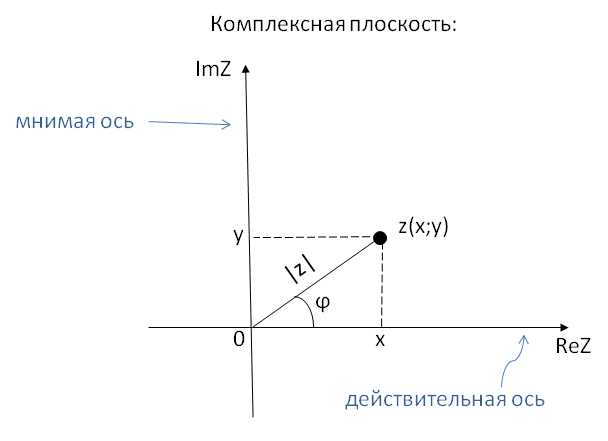
\includegraphics[scale=0.4]{complexplane1}

\[z = |z|(\cos  \varphi + i \sin  \varphi)\]
\[|z| = \sqrt{Re^2(z) + Im^2(z)} = \sqrt{x^2 + y^2}\]

Угол, который радиус-вектор образует с положительной осью $Re(z)$
называют аргументом $z$.

\[ \varphi = \textnormal{Arg}(z)\]
\[
    \begin{cases}
        \cos  \varphi = \frac{Re(z)}{|z|} \\
        \sin  \varphi = \frac{Im(z)}{|z|}
    \end{cases}
\]

При этом $ \varphi \in (-\pi; \pi]$ называют главным значением аргумента и обозначают $\arg z$
\[Arg(z) = \arg z + 2 \pi k, k \in \mathbb{Z}\]

\parspace

\underline{\textbf{Замечание}}

\begin{enumerate}
    \item Очевидно, $|Re(z)| \le |z|; |Im(z)| \le |z|$
    \item $|z|^2 = x^2 + y^2 = (x + iy)(x - iy) = z * \overline{z}$
    \item Из связи прямоугольной и полярной системы координат 
    
    $\implies Re(z) = |z| \cos (Arg(z)), Im(z) = |z| \sin (Arg(z)) \\
    z = Re(z) + i*Im(z) = |z|(\cos  \varphi + i \sin  \varphi)$ -- \textbf{тригонометрическая
    форма записи комплексного числа}.
\end{enumerate}

\subsection{Показательная форма записи комплексного числа}

Рассмотрим функцию Эйлера: $e^{i  \varphi} = \cos  \varphi + i \sin  \varphi$

\begin{theorem}[Свойства функции Эйлера]
    \begin{enumerate}
        \item $e^{i  \varphi_1} * e^{i  \varphi_2} = e^{i( \varphi_1 +  \varphi_2)}$
        \item $\frac{e^{i  \varphi_1}}{e^{i  \varphi_2}} = e^{i( \varphi_1 -  \varphi_2)}$
        \item $(e^{i  \varphi})^n = e^{i n  \varphi} \quad (n \in \mathbb{N})$
    \end{enumerate}    
\end{theorem}

\begin{proof}
    \begin{enumerate}
        \item
        \item
        \item
    \end{enumerate}    
\end{proof}

Введя функцию Эйлера: $z = |z| (\cos \varphi + i \sin \varphi), \quad z = |z| e^{i \varphi}$

\underline{\textbf{Замечание:}}

\begin{align*}
    z_1 &= |z_1| e^{i \varphi_1} \quad \varphi_1 = \textnormal{Arg} z i \\
    z_2 &= |z_2| e^{i \varphi_2} \\
    z_1 * z_2 &= |z_1| |z_2| e^{i (\varphi_1 + \varphi_2)} \\
    \frac{z_1}{z_2} &= \frac{|z_1|}{|z_2|} e^{i (\varphi_1 - \varphi_2)}, \, z_2 \ne 0 \\
    \textnormal{Arg} (z_1 * z_2) &= \textnormal{Arg} z_1 + \textnormal{Arg} z_2 \\
    \textnormal{Arg} (\frac{z_1}{z_2}) &= \textnormal{Arg} z_1 - \textnormal{Arg} z_2 \\
    \textnormal{Хотя } \textnormal{arg} (z_1 * z_2) &= \textnormal{Arg} z_1 + \textnormal{Arg} z_2 \textnormal{ не всегда}
\end{align*}

\underline{\textbf{Свойства $|z|$:}}

\begin{enumerate}
    \item $|z| \ge 0$
    \item $|z_1 * z_2| = |z_1| * |z_2|$
    
    $\left| \frac{z_1}{z_2} \right| = \frac{|z_1|}{|z_2|} \quad (z_2 \ne 0)$

    \item Неравенство $\triangle$
    
    $\left| |z_1| - |z_2| \right| \le |z_1 \pm z_2| \le |z_1| + |z_2|$
    
    $|z_1 \pm z_2|^2 = (z_1 \pm z_2) * \overline{(z_1 \pm z_2)} 
    = (z_1 \pm z_2) (\overline{z_1} \pm \overline{z_2})
    = z_1 * \overline{z_1} + z_2 * \overline{z_2} \pm (z_2 * \overline{z_2} + z_1 * \overline{z_1})
    = |z_1|^2+|z_2|^2 \pm 2 \real (z_2 * \overline{z_1})$

    $\real (z_2 * \overline{z_1}) \le |z_2 * \overline{z_1}| = |z_2| |\overline{z_1}| = |z_1| * |z_2|$

    $(|z_1|-|z_2|)^2 \le |z_1 \pm z_2| \le (|z_1| + |z_2|)^2
    = | |z_1| - |z_2| | \le |z_1 \pm z_2| \le |z_1| + |z_2|$
\end{enumerate}

\section{Сфера Римана}

Рассмотрим плоскость $XoY$ и касающуюся её в точке $O$ сферу
единичного диаметра. Точка $O$ -- южный полюс сферы, диаметрально
противоположный точке $P$ -- северному полюсу сферы. 

Возьмём комплексное число $Z$ на плоскости и пусть точка $M$ --
точка пересечения прямой $PZ$ и сферы.

Таким образом каждой точке плоскости можно сопоставить каждую точку 
сферы и, наоборот, каждой точке сферы (кроме $P$) можно сопоставить
каждую точку плоскости. Это соответствие называется стереографической
проекцией, а сфера -- \textbf{Сферой Римана}. 

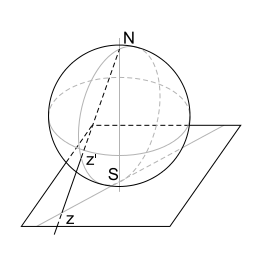
\includegraphics[scale=0.5]{riemannsphere}

Точке $P$ соответствует $z = \infty$ -- бесконечно удаленная точка.
Комплексную плоскость с бесконечно удаленной точкой $C$ называют
расширенную плоскостью и обозначают $\overline{\mathbb{C}}$.

\section{Векторы пространства $\mathbb{R}^m$}

\subsection{}

\begin{definition}
    Упорядоченную систему ($x_1, x_2, \dots, x_m$)($x_i \in \mathbb{R}$)
    (или ($z_1, z_2, \dots, z_m$); $z_i \in \mathbb{C}$) будем называть вектором
    (или точкой) пространства $\mathbb{R}^m (\mathbb{C}^m)$ если для этих
    систем определены понятия равенства и арифметические операторы сложения
    и умножения на число следующим образом:
    
    Имеем $u(u_1, u_2, \dots, u_m), v(v_1, v_2, \dots, v_m)$:
    
    \begin{enumerate}
        \item $u = v \Leftrightarrow u_i = v_i \quad \forall i = \overline{1, m}$
        \item $u + v = w$, где $w = (u_1 + v_1; u_2 + v_2; \dots; u_m + v_m)$
        \item $k \in \mathbb{R} (k \in \mathbb{C}) \\
        ku = w$, где $w = (k u_1, k u_2, \dots, k u_m)$
    \end{enumerate}
    
    Число $u_k$ называется $k$-й компонентой вектора $u$.
\end{definition}

\textbf{Свойства векторов}
\begin{enumerate}
    \item $u + v = v + u$
    \item $u + (v + w) = (u + v) + w$
    \item $u + v = u + w \Leftrightarrow v = w$
    \item $c * (u + v) = c * u + c * v \quad$ ($c$ -- const)
    \item $u * (c_1 + c_2) = u c_1 + u c_2 \quad$ ($c_1, c_2$ -- const)
    \item $c_1 * (c_2 * u) = (c_1 * c_2) * u \quad$ ($c_1, c_2$ -- const)
\end{enumerate}

\begin{definition}
    Скалярным произведением векторов $u(u_1, u_2, \dots, u_m), v(v_1, v_2, \dots, v_m)$
    называют число $u * v = \displaystyle\sum_{k = 1}^{m} u_k * \overline{v_k}$
\end{definition}

\textbf{Свойства скалярного произведения}
\begin{enumerate}
    \item $u * v = \overline{u * v}$
    \item $(\alpha u + \beta v) * w = \alpha (u * w) + \beta (v * w)$

    ($\alpha, \beta$ -- const)

    $u * (\alpha v + \beta w) = \overline{\alpha} (u * v) + \overline{\beta} (u * w)$

    \item $u * u \ge 0 \quad \forall u$, и $u * u = 0 \Leftrightarrow u = (0,0,\dots,0)$
\end{enumerate}

\begin{theorem}[Неравенство Коши-Буняковского]
    $|u v| \le \sqrt{(u * u) * (v * v)}$    
\end{theorem}

\begin{proof}
    Возьмём $\forall \lambda $ -- const

    \begin{enumerate}
        \item $(u + \lambda v) (u + \lambda v) \ge 0$
        \item $(u + \lambda v) u + \overline{\lambda} (u + \lambda v) v \ge 0$
        \item $(u * u) + \lambda (v * u) + \overline{\lambda} (u * v) + \overline{\lambda} * \lambda (v * v) \ge 0$
        \item $(u * u) + \lambda (v * u) + \overline{\lambda} (u * v) + |\lambda|^2 (v * v) \ge 0$
        \item Возьмём $\lambda = -\frac{(u * v)}{(v * v)} \quad (v \neq (0, \dots, 0))$
        \item $(u * u) - \frac{(u * v) (v * u)}{(v * v)} - \frac{\overline{(u * v)} (u * v)}{\overline{(v * v)}}
        + \frac{(u * v)^2}{(v * v)^2} (v * v) \ge 0$
        \item $(u * u) - 2 \frac{|(u * v)^2|}{(v * v)} + \frac{(u * v)^2}{(v * v)} \ge 0$
        \item $(u * u) - \frac{|u * v|^2}{(v * v)} \ge 0$
        \item $|u * v| \le \sqrt{(u * u) (v * v)}$
    \end{enumerate}
\end{proof}

\begin{definition}
    Модулем вектора $u$ называют число $|u| = \sqrt{(u * u)}$
\end{definition}

\textbf{Свойства модуля вектора}
\begin{enumerate}
    \item $|u_k| \le |u|$
    \item $|u * v| \le |u| * |v|$
    \item $\big||u| - |v|\big| \le |u \pm v| \le |u| + |v|$
\end{enumerate}

\parspace

\underline{\textbf{Замечание}}

Тогда в комплексном и векторном пространстве используемое понятие модуля
можно ввести аналогично понятиям окрестности, внутренней, изолированной,
предельной точке, замкнутого и открытого множества.

\section{Числовые последовательности}

\subsection{Числовые последовательности}

\begin{definition}
    Пусть $\forall n \in \mathbb{N}$ поставлено в соответствие единственное $x_n \in \mathbb{R}$,
    тогда говорят, что задана \textbf{числовая последовательность}, которую обозначают
    $\{x_n\}$, число $x_n$ называют $n$-ным членом последовательности.
\end{definition}

\begin{definition}
    Суммой, разностью, произведением, частным, линейной комбинацией последовательностей 
    $\{x_n\}$ и $\{y_n\}$ называется последовательность члены которой образуются 
    по следующим правилам соответственно: 
    $x_n + y_n; x_n - y_n; x_n * y_n; \frac{x_n}{y_n} (y_n \ne 0); \alpha x_n + \beta y_n (\alpha, \beta \in \mathbb{R})$.
\end{definition}

\begin{definition}
    $\{x_n\}$ называют ограниченной, если множество её элементов ограничено.
\end{definition}

\begin{definition}
    $\{x_n\}$ называют возрастающей (неубывающей, убывающей, невозрастающей), если
    $\forall n \in \mathbb{N} \quad x_n < x_{n + 1} (x_n \le x_{n + 1}; x_n > x_{n + 1}; x_n \ge x_{n + 1})$.
\end{definition}

\begin{definition}
    Последовательность $\{x_n\}$ называют сходящейся к числу $a$, а число $a$ называют
    \textbf{пределом} последовательности $\{x_n\}$ и обозначают 
    $\displaystyle\lim_{n \rightarrow \infty} x_n = a$, если 
    $\forall \varepsilon > 0 \quad \exists n_\varepsilon \in \mathbb{N}: \forall n \ge n_\varepsilon$
    выполняется неравенство $|x_n - a| < \varepsilon$.
\end{definition}

\underline{\textbf{Замечание}}.

$|x_n - a| < \varepsilon \Leftrightarrow -\varepsilon < x_n - a < \varepsilon 
\Leftrightarrow a - \varepsilon < x_n < a + \varepsilon
\Leftrightarrow x_n \in (a - \varepsilon; a + \varepsilon)$

\parspace

\underline{\textbf{Замечание}}.

$\displaystyle\lim_{x \rightarrow \infty} x_n = a$ означает, что
$\forall \varepsilon$-окрестностей точки $a$ найдется такой номер, 
начиная с которого все члены последовательности содержатся в этой
$\varepsilon$-окрестности точки $a$.

\begin{definition}
    $\{x_n\}$ называются бесконечно большой, если
    $\forall \varepsilon > 0 \quad \exists n_\varepsilon \in \mathbb{N}:
    \forall n \ge n_\varepsilon$ выполняется $|x_n| > \varepsilon$ и
    обозначается $\dslimn x_n = \infty$.
\end{definition}

\parspace

\underline{\textbf{Пример}}.

Докажем по определению 
$\dslimn \frac{1}{\sqrt[3]{n^2 + 1}} = 0$,
т.е. докажем, что $\forall \varepsilon > 0 \quad \exists n_\varepsilon \in \mathbb{N}:
\forall n \ge n_\varepsilon$ выполняется $\left|\frac{1}{\sqrt[3]{n^2 + 1}} - 0\right| < \varepsilon$
т.к. $\left|\frac{1}{\sqrt[3]{n^2 + 1}}\right| < \frac{1}{\sqrt[3]{n^2}}$,
а $\frac{1}{\sqrt[3]{n^2}} < \varepsilon \Leftrightarrow n > \frac{1}{\sqrt{\varepsilon^3}}
\implies$ если $\forall \varepsilon > 0$ выбрать 
$n_\varepsilon \in \mathbb{N}: n_\varepsilon > \frac{1}{\sqrt{\varepsilon^3}}$,
то $\forall n \ge n_\varepsilon$ выполняется $\left|\frac{1}{\sqrt[3]{n^2 + 1}} - 0\right| < \varepsilon$.

\begin{definition}
    Пусть дана $\{x_n\}$ и $\{k_n\}$-возрастающая последовательность натуральных чисел.
    Тогда $\{y_n\}: y_n = x_{k_n}$ называют подпоследовательностью последовательности $\{x_n\}$.
\end{definition}

\begin{definition}
    Если у $\{x_n\}$ существует подпоследовательность $\{y_n\}$ сходящаяся к числу $a^*$,
    то $a^*$ называют частичным пределом последовательности $\{x_n\}$.
    
    Наибольшим (наименьшим) из частичных пределов $\{x_n\}$ называют верхним (нижним) пределом
    и обозначают $\displaystyle\varlimsup_{n \to \infty} x_n$
    ($\displaystyle\varliminf_{n \to \infty} x_n$).
\end{definition}

\begin{theorem}[Больцано-Вейерштрасса для последовательностей]
    Всякая ограниченная последовательность имеет хотя бы один частичный предел.    
\end{theorem}
\begin{proof}
    $\{x_n\}$ -- ограниченная $\bydef$ множество $A$ её
    элементов ограничено.
    
    \underline{1 случай.} $A$ -- конечно.
    
    $\implies$ некоторому $a \in A$ соответствует бесконечное число элементов последовательности 
    \[x_{k_1} = 1, x_{k_2} = a, \dots, x_{k_n} = a, \dots\]
    \[(k_1 < k_2 < k_3 < \dots < k_n < \cdots)\]
    
    Получаем подпоследовательность $\{y_n\}: y_n = a (y_n = x_{k_n})$ и
    $\dslimn y_n = a \implies a$ -- частичный предел $\{x_n\}$.
    
    \underline{2 случай.} $A$ -- бесконечно (и ограничено).
    
    $\implies$ по \textit{Теореме Больцано-Вейерштрасса для множеств} у множества $A$
    существует предельная точка $x$.
    
    Возьмём числа $\varepsilon_n = \frac{1}{10^n}$ тогда по определению предельной точки
    в $\varepsilon_1$-окрестности точки $x$ найдется бесконечное количество элементов последовательности.
    
    Выберем $x_{k_1}$. В $\varepsilon_2$-окрестности точки $x$ найдется бесконечное
    количество элементов последовательности.
    
    Выберем $x_{k_2}: k_2 > k_1$.
    
    Повторим процесс.
    
    $\{x_{k_n}\}: \left| x_{k_n} - x \right| < \varepsilon_N \quad n \ge N$
    
    Тогда $\forall \varepsilon > 0$ выберем $\varepsilon_N < \varepsilon$
    (возьмём $N > \lg \frac{1}{\varepsilon}$) и $\forall n \ge N$ будем иметь 
    $\left| x_{k_n} - x \right| < \varepsilon$ 
    $\bydef \dslimn x_{k_n} = x$
    $\bydef x$ -- частичный предел последовательности $\{x_n\}$.    
\end{proof}

\underline{\textbf{Замечания}}.
\begin{enumerate}
    \item Тот факт, что $\{x_n\}$ не ограничено сверху (снизу) обозначается как 
    $\displaystyle\varlimsup_{n \to \infty} x_n = +\infty$ 
    ($\displaystyle\varliminf_{n \to \infty} x_n = -\infty$).

    \item Методом, предложенным в Теореме можно доказать, что определение точки
    эквивалентно другому определению: \textit{``Точка $x$ называется предельной точкой
    множества $A$, если существует последовательность, состоящая из элементов
    множества, сходящаяся к этой точке''}.
\end{enumerate}

\begin{theorem}[Свойства сходящихся последовательностей]
    \begin{enumerate}
        \item Если последовательность $\{x_n\} \underset{n \to \infty}{\to} a$,
        то любая её подпоследовательность $\underset{n \to \infty}{\to} a$.
    
        \item Сходящаяся последовательность может иметь только один предел.
        \item Если $\exists \dslimn x_n = a \ne 0 \implies
        \exists n_0 \in \mathbb{N} \quad \forall n \ge n_0$ $x_n$ имеет знак числа $a$.
    
        \item Сходящаяся последовательность ограничена.
        \item Если $\exists \dslimn x_n = x$ и
        $\exists \dslimn y_n = y \implies$
    
        $\exists \dslimn (\alpha x_n + \beta y_n) = \alpha x + \beta y$
        ($\alpha, \beta$ -- const)
    
        $\exists \dslimn (x_n y_n) = x y$
    
        $\exists \dslimn \frac{x_n}{y_n} = \frac{x}{y}$
        ($y_n \ne 0, y \ne 0$)
    
        \item Если $\forall n \ge n_0 \quad x_n \le y_n$ и 
        $\exists \dslimn x_n = x$ и
        $\exists \dslimn y_n = y$ $\implies x \le y$.
    
        \item Если $\forall n \ge n_0 \quad x_n \le y_n \le z_n$ и
        $\exists \dslimn x_n = 
        \dslimn z_n = a$
        $\implies \exists \dslimn y_n = a$
    \end{enumerate}
\end{theorem}
\begin{proof}
    \begin{enumerate}
        %--------------------------------------------------------------------------------------
        \item 
            По условию $\exists \dslimn x_n = a$
            $\bydef \underline{\forall \varepsilon > 0}
            \quad \underline{\exists n_\varepsilon \in \mathbb{N}}: 
            \forall n \ge \underline{n_\varepsilon}$ выполняется 
            $\left| x_n - a \right| < \varepsilon$. Но $\underline{k_n \ge n}$
            ($\{k_n\}$ -- возрастающая последовательность натуральных чисел)
            $\implies$ \underline{выполняется $\left| x_{k_n} - a \right| < \varepsilon$}
            $\implies$ $\dslimn x_{k_n} = a$.
    
        %--------------------------------------------------------------------------------------
        \item 
            \textit{От противного.} Пусть $\dslimn x_n = a$ и
            $\dslimn x_n = b \bydef$
            $\forall \varepsilon > 0 \begin{cases}
                \exists n_1 \in \mathbb{N}: \forall n \ge n_1 \quad \left| x_n - a \right| < \varepsilon \\
                \exists n_2 \in \mathbb{N}: \forall n \ge n_2 \quad \left| x_n - b \right| < \varepsilon
            \end{cases}$
        
            Выберем $n_3 = \max \left( n_1, n_2 \right)$, тогда начиная с номера $n_3$ будут выполняться оба
            неравенства одновременно.
        
            Рассмотрим $\left| a - b \right| = \left| a - x_n + x_n - b \right| = 
            \left| (a - x_n) + (x_n - b) \right| \le \left| x_n - a \right| + 
            \left| x_n - b \right| \underset{\forall n \ge n_3}{<}
            \varepsilon + \varepsilon = 2 \varepsilon$, т.е. $\left| a - b \right| < 2 \varepsilon$,
            при том, что $a - b$ -- неотрицательное число.
        
            Получаем, что неотрицательное число $<$ любого положительного 
            $\implies a - b = 0 \implies a = b$. \textbf{Противоречие.}
    
        %--------------------------------------------------------------------------------------
        \item 
            Имеем: $\exists \dslimn x_n = a \ne 0$
            $\bydef \forall \varepsilon > 0 \quad \exists n_\varepsilon \in \mathbb{N} 
            \forall n \ge n_\varepsilon$ выполняется $\left| x_n - a \right| < \varepsilon$
            или $a - \varepsilon < x_n < a + \varepsilon$.
            
            Возьмём $\varepsilon = \frac{\left| a \right|}{2} > 0 \implies 
            \exists n_0 \in \mathbb{N} \quad \forall n \ge n_0 \quad
            a - \frac{\left| a \right|}{2} < x_n < a + \frac{\left| a \right|}{2}$
        
            Отсюда получаем, что $x_n$ начиная с номера $n_0$ имеют тот же знак, что и число $a$.
    
        %--------------------------------------------------------------------------------------
        \item 
            Дано: $\dslimn x_n = a$
            $\bydef \forall \varepsilon > 0 \quad
            \exists n_\varepsilon \in \mathbb{N}: \forall n \ge n_\varepsilon \quad
            \left| x_n - a \right| < \varepsilon$.
        
            Возьмём $\varepsilon = 1 \implies \exists n_1 \in \mathbb{N}: \forall n \ge n_1 \quad
            \left| x_n - a \right| < 1$ или $a - 1 < x_n < a + 1$.
        
            Возьмём $m = \min \left( x_1, x_2, \dots, x_{n_1 - 1}, a - 1 \right)$.
        
            Возьмём $M = \min \left( x_1, x_2, \dots, x_{n_1 - 1}, a + 1 \right)$.
        
            $\implies \forall n \in \mathbb{N} \quad m \le x_n \le M$ $\implies \{x_n\}$ -- ограничена.
    
        %--------------------------------------------------------------------------------------
        \item 
            Дано:
            
            $\dslimn x_n = x$
            $\bydef \forall \varepsilon > 0 \quad
            \exists n_1 \in \mathbb{N}: \forall n \ge n_1 \quad
            \left| x_n - x \right| < \varepsilon$.
        
            $\dslimn y_n = y$
            $\bydef \forall \varepsilon > 0 \quad
            \exists n_2 \in \mathbb{N}: \forall n \ge n_2 \quad
            \left| y_n - y \right| < \varepsilon$.
        
            $\implies \forall n \ge n_3 = \max \left( n_1, n_2 \right)$ 
            выполняются оба неравенства одновременно.
        
            \begin{enumerate}[label*=\arabic*.]
                \item 
                    $|(\alpha x_n + \beta y_n) - (\alpha x + \beta y)| = 
                    |\alpha (x_n - x) + \beta (y_n - y)| \le 
                    |\alpha| |x_n - x| + |\beta| |y_n - y| 
                    \underset{\forall n \ge n_3}{<}
                    \underbrace{(|\alpha| + |\beta|) \varepsilon}_{\text{обозначим } \varepsilon^*} \\
                    \implies \forall \varepsilon^* > 0 \exists n_{\varepsilon^*} = n_3 \in \mathbb{N}:
                    \forall n \ge n_{\varepsilon^*}$ выполняется 
                    $|(\alpha x_n + \beta y_n) - (\alpha x + \beta y)| < \varepsilon^* \\
                    \bydef \dslimn (\alpha x_n + \beta y_n) = \alpha x + \beta y$
        
                \item 
                    Рассмотрим $|x_n y_n - x y| = |x_n y_n - x y_n + x y_n - x y| = 
                    |(x_n y_n - x y_n) + (x y_n - x y)| = 
                    |(x_n - x) y_n + x (y_n - y)| \le |x_n - x| |y_n| + |x| |y_n - y| \quad (1)$
            
                    Но $\{y_n\}$ сходится $\stackrel{\text{по св 4}}{\implies} \{y_n\}$ -- ограничена
                    $\implies \exists C > 0 \quad \forall n \in \mathbb{N} \quad |y_n| \le C$.
            
                    $\implies (1) \underset{\forall n \ge n_3}{<} 
                    \underbrace{\varepsilon (C + |x|)}_{\varepsilon^*} \implies
                    \forall \varepsilon^* > 0 \quad \exists n_{\varepsilon^*} = n \in \mathbb{N}:
                    \forall n \ge n_{\varepsilon^*} \quad |x_n y_n - x y| < \varepsilon^*$.
        
                \item 
                    $\left| \frac{x_n}{y_n} - \frac{x}{y} \right| = 
                    \left| \frac{x_n y - x y_n}{y_n y} \right| =
                    \left| \frac{x_n y - x y + x y - x y_n}{y_n y} \right| =
                    \left| \frac{y (x_n - x) + x (y - y_n)}{y_n y} \right| \stackrel{\triangle}{\le}
                    \frac{|x_n - x}{y_n} + \frac{|x|}{|y_n| |y|} |y_n - y| \quad (2)$
            
                    Так как $\{y_n\}$ сходится, то для 
                    $\varepsilon = \frac{|y|}{2} \quad \exists n_4 \in \mathbb{N} \quad
                    \forall n \ge n_4$ выполняется $|y_n - y| < \frac{|y|}{2} \implies
                    \left| |y_n| - |y| \right| < \frac{|y|}{2} \implies
                    |y_n| > |y| - \frac{|y|}{2} \implies \frac{1}{|y_n|} < \frac{2}{|y|}$.
            
                    $\implies (2) < \underbrace{\varepsilon ( \frac{2}{|y|} + \frac{|x|}{ (|y| - 1) |y| } )}_{\varepsilon^*}
                    \implies \forall \varepsilon^* > 0 \quad 
                    \exists n_{\varepsilon^*} = \max (n_3, n_4) \in \mathbb{N}:
                    \forall n \ge n_4$ выполняется 
                    $\left| \frac{x_n}{y_n} - \frac{x}{y} \right| < \varepsilon^* 
                    \implies \dslimn \frac{x_n}{y_n} = \frac{x}{y}$.
            \end{enumerate}
    
        %--------------------------------------------------------------------------------------
        \item 
            Имеем $\forall n \ge n_0 \quad x_n \le y_n \quad 
            \exists \dslimn x_n = x 
            \bydef \forall \varepsilon > 0 \quad
            \exists n_1 \in \mathbb{N} \quad \forall n \ge n_1 \quad |x_n - x| < \varepsilon$
            и $\exists \dslimn y_n = y 
            \bydef \forall \varepsilon > 0 \quad
            \exists n_2 \in \mathbb{N} \quad \forall n \ge n_2 \quad |y_n - y| < \varepsilon$
        
            Возьмём $n_3 = \max (n_0, n_1, n_2) \implies \forall n \ge n_3$ выполняются
            все три неравенства одновременно.
        
            Пусть \textit{от противного} $x > y$. 
            $x_n - y_n = (x_n - x) - (y_n - y) + (x - y) > 
            -\varepsilon - \varepsilon + (x - y) = (x - y) - 2 \varepsilon$, где $(x - y) > 0$.
        
            Тогда неравенство будет верным, если $2 \varepsilon < (x - y) \implies x_n > y_n$,
            а \textbf{это противоречит условию} $\implies x \le y$.
    
        %--------------------------------------------------------------------------------------
        \item 
            Дано: $\forall n \ge n_0 \quad x_n \le y_n \le z_n, 
            \dslimn x_n = a \bydef
            \forall \varepsilon > 0 \quad \exists n_1 \in \mathbb{N}:
            \forall n \ge n_1 \quad |x_n - a| < \varepsilon$ или
            $-\varepsilon < x_n - a < \varepsilon$.
            
            $\dslimn z_n = a \bydef
            \forall \varepsilon > 0 \quad \exists n_2 \in \mathbb{N}:
            \forall n \ge n_2 \quad |z_n - a| < \varepsilon$ или
            $-\varepsilon < z_n - a < \varepsilon$.
        
            Тогда $\forall n \ge n_3 = \max (n_1, n_2, n_0)$ оба неравенства
            будут выполняться одновременно.
        
            $\underline{-\varepsilon} < x_n - a \le \underline{y_n - a} \le
            z_n - a < \underline{\varepsilon} \Leftrightarrow |y_n - a| < \varepsilon
            \implies \forall \varepsilon > 0 \quad \exists n_\varepsilon = n_3 \in \mathbb{N}:
            \forall n \ge n_3 \quad |y_n - a| < \varepsilon \bydef 
            \dslimn y_n = a$.
    \end{enumerate}
\end{proof}

\begin{theorem}[Свойства верхнего (и нижнего) предела последовательности]
    Если $\exists \displaystyle\varlimsup_{n \to \infty} x_n = a$ 

    или ($\exists \displaystyle\varliminf_{n \to \infty} x_n = a$)
    $\implies \forall \varepsilon > 0$ существует лишь конечное число элементов
    последовательности превосходящие $(a + \varepsilon)$ (меньше $(a - \varepsilon)$).
\end{theorem}
\begin{proof}
    \textbf{ДОКАЗАТЬ ДЛЯ СЛУЧАЯ В СКОБКАХ!!!}

    Пусть $\exists \displaystyle\varlimsup_{n \to \infty} x_n = a$ и $\varepsilon > 0$ и
    пусть \textit{от противного} найдется бесконечное число элементов больших, чем
    $(a + \varepsilon)$. Составим из них новую последовательность. Тогда по 
    \textit{свойству 6 теоремы (свойства сходящихся последовательностей)} любой
    частичный предел этой последовательности будет $\ge (a + \varepsilon)$.
    
    Но он является и частичным пределом исходной последовательности, причём $> a$, но
    это противоречит тому, что $a$ -- верхний предел $\implies$ таких элементов может
    быть только конечное число.
\end{proof}

\begin{definition}
    Последовательность $\{x_n\}$ называется фундаментальной, если 
    $\forall \varepsilon > 0 \quad \exists n_\varepsilon \in \mathbb{N}:
    \forall n \ge n_\varepsilon \quad \forall m \ge n_\varepsilon$
    выполняется $|x_n - x_m| < \varepsilon$.
\end{definition}

\begin{theorem}[Критерий Коши сходимости последовательности]
    Пусть $\{x_n\}$ сходится $\Leftrightarrow$ $\{x_n\}$ фундаментальна.    
\end{theorem}
\begin{proof}
    \begin{enumerate}
        \item 
            Сходится $\implies$ фундаментальна.
            
            По условию $\{x_n\}$ сходится $\implies \exists \dslimn x_n = a
            \implies \underline{\forall \varepsilon > 0 \quad \exists n_\varepsilon \in \mathbb{N} \quad \forall n \ge n_\varepsilon}$
            выполняется $|x_n - a| < \frac{\varepsilon}{2}$ и для $\underline{\forall m \ge n_\varepsilon}$ 
            выполняется $|x_m - a| < \frac{\varepsilon}{2}$.
        
            Рассмотрим $\underline{|x_n - x_m|} = |(x_n - a) + (a - x_m)| 
            \le |x_n - a| + |x_m - a| \le \frac{\varepsilon}{2} + \frac{\varepsilon}{2} = \varepsilon
            \bydef \{x_n\}$ -- фундаментальна.
    
        \item
            Фундаментальна $\implies$ сходится.
            
            Имеем $\{x_n\}$ -- фундаментальна 
            $\implies \forall \varepsilon > 0 \quad \exists n_\varepsilon \in \mathbb{N}:
            \forall n \ge n_\varepsilon \quad \forall m \ge n_\varepsilon$ выполняется
            $|x_n - x_m| < \varepsilon$.
        
            Тогда для $\varepsilon = 1 \quad \exists n_1 \in \mathbb{N} \quad 
            \forall n \ge n_1 \quad \forall m \ge n_1$ выполняется $|x_n - x_m| < 1$
        
            Зафиксируем $m: m \ge n_1$.
        
            $|x_n| = |(x_n - x_m) + x_m| \le |x_n - x_m| + |x_m| < 
            \underbrace{1 + |x_m|}_{C \text{ -- const}} \quad \forall n \ge n_1$
            $\implies \{x_n\}$ -- ограничена $\implies$ по 
            \textit{Теореме Больцано-Вейерштрасса для последовательностей} у $\{x_n\}$
            существует хотя бы один частичный предел, т.е. 
            $\exists \{x_{k_n}\} \underset{n \to \infty}{\to} x$
            $\bydef$ для нашего $\varepsilon > 0 \quad \exists k_{n_\varepsilon} \in \mathbb{N}:
            \forall k_n \ge k_{n_\varepsilon}$ выполняется $|x_{k_n} - x| < \varepsilon$.
        
            Рассмотрим $\forall n \ge k_{n_\varepsilon} \ge n_\varepsilon:
            |x_n - x| = |(x_n - x_{k_n}) + (x_{k_n} - x)| \le |x_n - x_{k_n}| + |x_{k_n} - x|
            < \underbrace{2 \varepsilon}_{\varepsilon^*}$.
        
            Получим:
            $\forall \varepsilon^* \quad \exists n_{\varepsilon^*} = n_\varepsilon \in \mathbb{N}:
            \forall n \ge n_{\varepsilon^*}$ имеем $|x_n - x| < \varepsilon^*$
            $\bydef \exists \dslimn x_n = x$
    \end{enumerate}
        
\end{proof}

\begin{theorem}[Признак сходимости монотонной последовательности]
    Ограниченная сверху (снизу) неубывающая (возрастающая) последовательность сходится.
\end{theorem}

\begin{proof}
    \textbf{ДОКАЗАТЬ ДЛЯ СЛУЧАЯ В СКОБКАХ!!!}

    $\{x_n\}$ -- неубывающая и ограниченная сверху $\implies$ множество элементов
    $\{x_n\}$ ограничено сверху $\implies$ по
    \textit{Теореме О существовании верхней грани} 
    $\exists \sup x_n \stackrel{\text{об.}}{=} a$ $\implies$ по признаку:
    \begin{enumerate}
        \item $\forall n \in \mathbb{N} \quad x_n \le a$
        \item $\forall \varepsilon > 0 \quad 
        \exists x_{n_\varepsilon} : x_{n_\varepsilon} > a - \varepsilon$
    \end{enumerate}
    
    Возьмём $n \ge n_\varepsilon$: 
    $a - \varepsilon < x_{n_\varepsilon} \le x_n \le a < a + \varepsilon
    \implies \forall \varepsilon > 0 \quad \exists n_\varepsilon \in \mathbb{N}:
    \forall n \ge n_\varepsilon$ выполняется $a - \varepsilon < x_n < a + \varepsilon$
    или $|x_n - a| < \varepsilon \bydef \exists \dslimn x_n = a$.
\end{proof}

\subsection{Замечательные пределы}

\begin{enumerate}
    \item 
        $\displaystyle \lim_{n \to \infty} \left( 1 + \frac{1}{n} \right)^n = e$ (Второй замечательный предел)
        
        Рассмотрим $x_n = \left( 1 + \frac{1}{n} \right)^{n + 1}$. 
        Имеем $x_n > 1 \quad \forall n \in \mathbb{N}$ $\implies \{x_n\}$ -- ограничена снизу.

        Рассмотрим $\frac{x_n}{x_{n-1}} = 
        \frac{\left( 1 + \frac{1}{n} \right)^{n - 1}}{\left( 1 + \frac{1}{n - 1} \right)^{n}}
        = \frac{(n + 1)^{n+1} * (n - 1)^n}{n^{n+1} * n^n}
        = \left( \frac{(n + 1) * (n - 1)}{n^2} \right)^n * \frac{n + 1}{n}
        = \left( 1 - \frac{1}{n^2} \right)^{n} * \left( 1 + \frac{1}{n} \right)
        \le \left( 1 - \frac{1}{n^2} \right)^{n} * \left( 1 + \frac{1}{n^2} \right)^n
        \le \left( 1 - \frac{1}{n^4} \right)^{n} < 1 \implies x_n < x_{n-1}$

        Т.е. $\{x_n\}$ -- убывающая последовательность $\implies$
        по \textit{Теореме О сходимости монотонной последовательности}
        $\exists \dslimn x_n = 
        \dslimn \left( 1 + \frac{1}{n} \right)^{n + 1} = e$

        $\dslimn \left( 1 - \frac{1}{n} \right)^{n}
        = \dslimn \frac{x_n}{1 + \frac{1}{n}} = e \approx 2.71828$

    %%%%%%%%%%%%%%%%%%%%%%%%%%%%%%%%%%%%%%%%%%%%

    \item 
        Докажем, что $\dslimn \frac{n^k}{a^n} = 0,
        \quad k \in \mathbb{N}, \quad a > 1$

        $\dslimn \frac{n^k}{a^n} = 
        \dslimn \left( \frac{n}{(\sqrt[k]{a})^n} \right)^k$

        Рассмотрим $(\sqrt[k]{a})^n = (1 + (\sqrt[k]{a} - 1)) ^ n = 
        1 + n * (\sqrt[k]{a} - 1) + \frac{n (n - 1)}{2} (\sqrt[k]{a} - 1)^2
        + \dots + (\sqrt[k]{a} - 1)^n > \frac{n (n - 1)}{2} (\sqrt[k]{a} - 1)^2$

        Получаем $(\sqrt[k]{a})^n > \frac{n (n - 1)}{2} (\sqrt[k]{a} - 1)^2$

        $\implies$ по \textit{$7^{\text{о}}$ свойству сходящихся последовательностей}
        $\dslimn \frac{n}{(\sqrt[k]{a})^n} = 0
        \implies \dslimn \frac{n^k}{a^n} = 0$

    %%%%%%%%%%%%%%%%%%%%%%%%%%%%%%%%%%%%%%%%%%%%

    \item 
        $\dslimn \frac{a^n}{n!} = 0, \quad a > 0$

        $0 < \underbrace{\frac{a}{1} * \frac{a}{2} * \frac{a}{3} * \dots * \frac{a}{k_0 - 1}}_A
        * \underbrace{\frac{a}{k_0}}_{\frac{a}{k_0} = q < 1}
        * \frac{a}{k_0 + 1} * \dots *
        \frac{a}{n} < A * q^{n - k_0 + 1}$

        $\implies$ по \textit{$7^{\text{о}}$ свойству сходящихся последовательностей}
        $\dslimn \frac{a^n}{n!} = 0$

    %%%%%%%%%%%%%%%%%%%%%%%%%%%%%%%%%%%%%%%%%%%%
    
    \item 
        $\dslimn \sqrt[n]{n} = 1$
        
        При $n > 1: \sqrt[n]{n} > 1 \implies \sqrt[n]{n} = 1 + \beta_n \implies
        n = (1 + \beta_n)^n = 1 + n \beta_n + \frac{n (n - 1)}{2} (\beta_n)^2 + \dots +
        (\beta_n)^n > \frac{n (n - 1)}{2} (\beta_n) ^ 2 \implies
        0 < \beta_n < \sqrt{\frac{2}{n-1}} \implies
        \dslimn \beta_n = 0 \implies
        \dslimn \sqrt[n]{n} = 1$
\end{enumerate}

\section{Последовательности комплексных чисел}

\subsection{Последовательности комплексных чисел}

\textbf{Последовательности комплексных чисел} аналогично определение последовательности
действительных чисел.

Определение \textit{сходимости} даётся аналогично.

Определение \textit{частичного предела сохраняется}.

Понятия \textit{верхнего, нижнего предела} и \textit{монотонности} для комплексных
чисел не имеют смысла.

\begin{theorem}[О связи сходимости $\{z_n\}$ со сходимостью $\{\real z_n\}$ и $\{\imagin z_n\}$.]
    Если $\exists \dslimn z_n = \alpha + i \beta
    \implies \begin{cases}
        \exists \dslimn \real z_n = \alpha \\
        \exists \dslimn \imagin z_n = \beta
    \end{cases}$        
\end{theorem}

\begin{proof}
    \begin{enumerate}
        \item
            $\exists \dslimn z_n = \alpha + i \beta \; (z_n = x_n + i y_n)
            \bydef \forall \varepsilon > 0 \quad \exists n_\varepsilon \in \mathbb{N}:
            \forall n \ge n_\varepsilon$ выполняется $|z_n - (\alpha + i \beta)| < \varepsilon$
            или $|(x_n- \alpha) + i (y_n - \beta)| < \varepsilon$
        
            Но $|x_n - \alpha| \le |(x_n - \alpha) + i (y_n - \beta)| < \varepsilon
            \bydef \exists \dslimn x_n = \alpha$
        
            Но $|y_n - \beta| \le |(x_n - \alpha) + i (y_n - \beta)| < \varepsilon
            \bydef \exists \dslimn y_n = \beta$
    
        \item 
            $\exists \dslimn x_n = \alpha, \; \exists \dslimn y_n = \beta
            \bydef \forall \varepsilon > 0 \begin{cases}
                \exists n_1 \in \mathbb{N} \quad \forall n \ge n_1 \quad |x_n - \alpha| < \frac{\varepsilon}{\sqrt{2}} \\
                \exists n_2 \in \mathbb{N} \quad \forall n \ge n_2 \quad |y_n - \alpha| < \frac{\varepsilon}{\sqrt{2}}
            \end{cases}$
            
            $n_3 = \max (n_1, n_2) \implies \forall n \ge n_3:
            |z_n - (\alpha + i \beta)| = |(x_n - \alpha) + i (y_n - \beta)| =
            \sqrt{(x_n - \alpha)^2 + (y_n - \beta)^2} <
            \sqrt{\frac{\varepsilon^2}{2} + \frac{\varepsilon^2}{2}} = \varepsilon$
        
            Получаем $\forall \varepsilon > 0 \quad \exists n_\varepsilon = n_3 \in \mathbb{N}:
            \forall n \ge n_3$ выполняется $|z_n - (\alpha + i \beta)| < \varepsilon
            \implies \dslimn z_n = \alpha + i \beta$
    \end{enumerate}
\end{proof}

\begin{theorem}[О связи сходимости $\{z_n\}$ со сходимостью $\{|z_n|\}$.]
    Если $\exists \dslimn z_n = A \implies \exists \dslimn |z_n| = |A|$
\end{theorem}

\begin{proof}
    $\dslimn z_n = A \implies \forall \varepsilon > 0 \quad \exists n_\varepsilon \in \mathbb{N}:
    \forall n \ge n_\varepsilon$ выполняется $||z_n| - |A|| \le |z_n - A| < \varepsilon
    \bydef \exists \dslimn |z_n| = |A|$
\end{proof}

\underline{\textbf{Замечания}}
\begin{enumerate}
    \item Про последовательность аргументов без дополнительных условий мы такую
    теорему высказать не можем.

    \item Теорема \textit{О свойствах сходящихся последовательностей} переносится
    и на комплексные числа за исключением свойств. $\prop{3}, \prop{6}, \prop{7}$.

    \item Для последовательностей векторов пространства $\mathbb{R}^n$ аналогично
    вводится определение последовательности, сходимости последовательности,
    также, как и для комплексных чисел справедлива Теорема, что если
    $\exists \dslimn u_n = A, \; u_n = (u_1^n, \dots, u_m^n), \;
    A = (a_1, \dots, a_m) \implies \exists \dslimn u_k^n = a_k \quad 
    \forall k = \overline{1, m}$

    а также свойства ??? справедливы, за исключением тех, что связаны
    с операциями $>, <$ или деления.
\end{enumerate}

\section{Пределы функций}

\subsection{Пределы функций}

\begin{definition}
    Если каждому $x \in A$ поставить в соответствие единственное число $y \in B$,
    то говорят, что это соответствие задаёт функцию $y = f(x)$.

    Множество $A$ называют \textit{областью определения функции} и обозначают $D_f$.

    Множество $B$ называют \textit{областью значений функции} и обозначают $E_f$.

    $x$ -- аргумент, $y = f(x)$ -- значение функции в точке $x$.
\end{definition}

\parspace

\textbf{Примеры:}
\begin{enumerate}
    \item $A \subset \R, B \subset \R \quad y = f(x)$ -- действительная
    функция действительного аргумента

    \item $A \subset \bb{C}, B \subset \bb{C} \quad w = f(z)$ -- комплексная
    функция комплексного аргумента.

    \item $A \subset \R^m, B \subset \R \quad y = f(x_1, \dots, x_m)$ --
    действительная функция многих переменных.

    \item $A \subset \R^m, B \subset \R^n \quad 
    (y_1, \dots, y_n) = (f_1(x_1, \dots, x_m), f_2(x_1, \dots, x_m), \dots, f_n(x_1, \dots, x_m))$ --
    векторная функция векторного аргумента.
\end{enumerate}

\begin{definition}
    Функция $y = f(x)$ называется ограниченой (сверху, снизу), если её множество
    значений ограничено (сверху, снизу), т.е 
    \[
        \exists m, M: \, \forall x \in D_f \quad m \le f(x) \le M
        \text{ или }
        \exists C: \, \forall x \in D_f \quad  | f(x) | \le C
        \; \text{(ограничено)}
    \]

    \[\exists M: \, \forall x \in D_f \quad f(x) \le M \; \text{(огр. сверху)}\]

    \[\exists m: \, \forall x \in D_f \quad m \le f(x) \; \text{(огр. снизу)}\]
\end{definition}

Пусть функция $y = f(x)$ задана на множестве $A$ и $a$ -- предельная точка $A$.

\begin{definition}[предела функции по Гейне]
    Число $b$ называют пределом функции $f(x)$ в точке $a$ \textbf{в смысле Гейне}
    и обозначают $\dslim_{x \to a} f(x) = b$, если
    $\forall \{ x_n \}: x_n \in A, x_n \ne a, x_n \approach{n \to \infty} a$ выполняется
    $f(x_n) \approach{n \to \infty} b$, то $b$ -- предел функции $f$ в точке $a$.
\end{definition}

\begin{definition}[предела функции по Коши]
    Число $b$ называют пределом функции $f(x)$ в точке $a$ \textbf{в смысле Коши}
    и обозначают $\dslim_{x \to a} f(x) = b$, если
    $\forall \varepsilon > 0 \quad \exists \delta_\varepsilon > 0 \quad
    \forall x \in A : \; 0 < | x - a | < \delta_\varepsilon$ выполняется
    $|f(x) - b| < \varepsilon$

    *рисунок*
\end{definition}

\begin{theorem}[Об эквивалентности определений Коши и Гейне]
    Определение Коши и Гейне предела функции в точке эквивалентны.
\end{theorem}
\begin{proof}
    \begin{enumerate}[label=\alph*)]
        \item 
            Пусть $b = \dslim_{x \to a} f(x)$ в смысле Коши.
            $\bydef$ $\forall \varepsilon > 0 \quad 
            \exists \delta_\varepsilon > 0 \quad \forall x \in A: \; 0 < |x - a| < \delta_\varepsilon$
            выполняется $|f(x) - b| < \varepsilon$.

            Возьмём $\forall \{ x_n \}: x_n \in A, x_n \ne a, \dslimn x_n = a$
            $\bydef$ $\forall \delta > 0 \quad \exists n_\delta \in \N: 
            \forall n \ge n_\delta$ выполняется $| x_n - a | < \delta$

            Возьмём $\delta = \delta_\varepsilon$ и тогда имеем, что $0 < |x_n - a| < \delta_\varepsilon$

            Тогда получим, что $|f(x_n) - b| < \varepsilon \implies 
            \forall \varepsilon > 0 \quad \exists n_\varepsilon = n_\delta \in \N \quad
            \forall n \ge n_\varepsilon$ выполняется $|f(x_n) - b| < \varepsilon
            \bydef \exists \dslim_{n \to b} f(x_n) = b \implies b = \dslim_{x \to a} f(x)$
            в смысле Гейне.

        \item
            Пусть $b = \dslim_{x \to a} f(x)$ в смысле Гейне.
            $\bydef$ $\forall \{ x_n \}: x_n \in A, x_n \ne a, \dslimn x_n = a$
            выполняется $f(x_n) \approach{n \to \infty} b$.

            \textit{Допустим от противного}, $b$ не является пределом $f(x)$ в точке $a$ в смысле Коши:
            $\forall \varepsilon_0 > 0 \quad \forall \delta > 0 \quad \exists x_0 \in A: \; 0 < |x_0 - a| < \delta$,
            но $|f(x_0) - b| \ge \varepsilon_0$

            Возьмём
            \[\delta = 1 \implies \exists x_1 \in A: \; 0 < |x_1 - a| < 1 \text{, но } |f(x_1) - b| \ge \varepsilon_0\]
            \[\delta = \frac{1}{2} \implies \exists x_2 \in A: \; 0 < |x_2 - a| < \frac{1}{2} \text{, но } |f(x_2) - b| \ge \varepsilon_0\]
            \[\dots\]
            \[\delta = \frac{1}{n} \implies \exists x_n \in A: \; 0 < |x_n - a| < \frac{1}{n} \text{, но } |f(x_n) - b| \ge \varepsilon_0\]
            \[\dots\]

            Получим $\{ x_n \}: x \in A, x_n \ne 0$ и $0 < |x_n - a| < \frac{1}{n}$, т.е.
            $x_n \approach{n \to \infty} a$, но
            $f(x_n)$ \cancel{$\approach{n \to \infty}$} $b$ (т.к. $|f(x_n) - b| \ge \varepsilon_0$),
            т.е. определение Гейне не выполняется.

            Получили противоречие $\implies$ $b$ является пределом $f(x)$ в точке $a$ в смысле Коши.
    \end{enumerate}
\end{proof}

\begin{theorem}[Критерий Коши предела функции в точке]
    Для того, чтобы существовал $\dslim_{x \to a} f(x)$ необходимо и достаточно, чтобы
    $\forall \eps > 0 \quad \exists \delta_\eps > 0: \forall x' \in A, x'' \in A:
    \begin{array}{c}
        0 < | x' - a | < \delta_\eps \\
        0 < | x'' - a | < \delta_\eps
    \end{array}$ выполняется $| f(x') - f(x'') | < \eps$.
\end{theorem}
\begin{proof}
    \begin{enumerate}[label=\alph*)]
        \item 
            Необходимость

            Имеем, что $\exists \dslim_{x \to a} f(x) = b$ $\implies$ по определению Коши
            $\forall \eps > 0 \quad \exists \delta_\eps > 0: \forall x \in A: 0 < | x - a | < \delta_\eps$
            выполняется $| f(x) - b | < \frac{\eps}{2}$

            Возьмём $x', x'' \in A:
            \begin{array}{c}
                0 < | x' - a | < \delta_\eps \\
                0 < | x'' - a | < \delta_\eps
            \end{array}$

            Тогда $| f(x') - b | < \frac{\eps}{2}$ и $| f(x'') - b | < \frac{\eps}{2}$

            Рассмотрим $| f(x') - f(x'') | = | (f(x') - b) + (b - f(x'')) | \stackrel{\triangle}{\le}
            | f(x') - b | + | f(x'') - b | < \eps$.

            Получили что и требовалось доказать.
        
        \item
            Достаточность

            Пусть $\forall \eps > 0 \quad \exists \delta_\eps > 0: \forall x', x'' \in A:
            \begin{array}{c}
                0 < | x' - a | < \delta_\eps \\
                0 < | x'' - a | < \delta_\eps
            \end{array}$ выполняется $| f(x') - f(x'') | < \eps$

            Возьмём $\forall \{ x_n \}: \: x_n \in A, x_n \ne a, x_n \approach{n \to \infty} a$
            $\implies$ по критерию Коши $\forall \delta > 0 \quad \exists n_\delta \in \N:
            \forall n \ge n_\delta, \forall m \ge n_\delta$ выполняется $| x_n - x_m | < \delta$.

            Возьмём $\delta = \delta_\eps, x' = x_n, x'' = x_m \implies | x' - x'' | < \delta$.

            Если использовать определение предела, то есть для $\delta > 0 \quad \exists n_{\delta^*} \in \N:
            \begin{array}{c}
                \forall n \ge n_{\delta^*} \text{ выполняется } | x_n - a | < \delta \\
                \forall m \ge n_{\delta^*} \text{ выполняется } | x_m - a | < \delta
            \end{array}$

            $\delta = \delta_\eps, x' = x_n, x'' = x_m$ выполняется
            $\begin{array}{c}
                0 < |x' - a| < \delta_\eps \\
                0 < |x'' - a| < \delta_\eps
            \end{array}$
            $\implies |f(x') - f(x'')| < \eps$ или $|f(x_n) - f(x_m)| < \eps$.
            
            Получили, что $\forall \eps > 0 \quad \exists n_\eps = n_{\delta^*} \in \N: \:
            \forall n \ge n_\eps$ выполняется $|f(x_n) - f(x_m)| < \eps \implies
            \{ f(x_n) \}$ -- фундаментальна $\implies \{ f(x_n) \}$ -- сходится и пусть
            $b = \dslimn f(x_n)$.

            Осталось доказать, что $b$ не зависит от выбора $\{ x_n \}$.

            Пусть $x'_n \approach{} a, x_n'' \approach{} a$. Сопоставим последовательность
            $x'_1, x''_1, x'_2, x''_2, \dots, x'_n, x''_n: \: y_n \implies y_n \approach{} a
            \implies f(y_n)$ -- сходится.

            Но если $\dslimn f(x'_n) = b \implies \dslimn f(x''_n) = b \implies b = \dslim_{x \to a} f(x)$
            в смысле Гейне.
    \end{enumerate}
\end{proof}

\begin{definition}
	Число $b$ называется левым (правым) пределом функции $f(x)$ в точке $x = a$, 
    если $\forall \eps > 0 \quad \exists \delta_\eps > 0: \: \forall x \in A: \: a - \delta_\eps < x < a$ 
    выполняется $|f(x) - b| < \eps \quad (a < x < a + \delta_\eps)$ и обозначается 
    $b = \dslim_{x \to a - 0} f(x) \quad (b = \dslim_{x \to a + 0} f(X))$
\end{definition}

\textbf{Утверждение. }
$\exists \dslim_{x \to a} f(x) - b \iff \exists \dslim_{x \to a - 0} = \dslim_{x \to a + 0} = b$

\begin{definition}
    Пусть $\omega(\omega_1, \omega_2, \dots, \omega_m) \in R^m$ -- произвольный вектор
    единичной длины $|\omega|=1$ и пусть в любой окрестности точки $a \in R^m$ имеются 
    точки вида $x(t) = a + t \omega$ ($t \in R,\, 0 \le t \le t_0$), входящие в область определения $f(x)$.
    Для таких $x(t)$ рассмотрим функцию $ \varphi(t) = f(x(t))$. Если $\exists \dslim_{t \to 0 + 0}  \varphi(t) = b$,
    то его называют пределом $f(x)$ в точке $x = a$ по направлению вектора $\omega$.
\end{definition}


*Рисунок*

\begin{example}
    Если $\exists \dslim_{x \to a} f(x) \quad (x \in R^m) \implies f(x)$ 
    имеет в точке a предел по любому направлению, обратное - неверно!

    Рассмотрим $u(x_1, x_2) = \frac{x_1^2-x_2^2}{x_1^2+x_2^2}; \quad a(0, 0)$

    $\forall\omega \implies$

    \[ x(t) = (t \omega_1; t \omega_2) \]
    \[ 
         \varphi(t) = u(x(t)) = 
        \frac{(t \omega_1)^2 - (t \omega_2)^2}{(t \omega_1)^2 + (t \omega_2)^2} = 
        \frac{t^2 (\omega_1^2 - \omega_2^2)}{t^2 (\omega_1^2 + \omega_2^2)}
    \]
    \[
        \implies \exists \dslim_{t \to +0}  \varphi(t) = 
        \dslim_{t \to +0} \frac{t^2 (\omega_1^2 - \omega_2^2)}{t^2 (\omega_1^2 + \omega_2^2)} = 
        \frac{\omega_1^2 - \omega_2^2}{\omega_1^2 + \omega_2^2}
    \]

    Но для каждого направления этот предел свой $\implies \not\exists \dslim_{x \to a} u(x)$  
\end{example}

\begin{definition}
    Будем обозначать: 
    \begin{enumerate}
        \item $\dslim_{x \to a} f(x) = \infty \iff \forall \eps > 0 \quad \exists \delta_\eps > 0 \quad \forall x \in A:\: 0 < |x-a| < \delta_\eps$ выполняется $|f(x)| > \eps$
        \item $\dslim_{x \to a} f(x) = +\infty \iff \forall \eps > 0 \quad \exists \delta_\eps > 0 \quad \forall x \in A:\: 0 < |x-a| < \delta_\eps$ выполняется $f(x) > \eps$
        \item $\dslim_{x \to a} f(x) = -\infty \iff \forall \eps > 0 \quad \exists \delta_\eps > 0 \quad \forall x \in A:\: 0 < |x-a| < \delta_\eps$ выполняется $f(x) < -\eps$
        \item $\dslim_{x \to \infty} f(x) = b \iff \forall \eps > 0 \quad \exists \delta_\eps > 0 \quad \forall x \in A:\: |x| > \delta_\eps$ выполняется $|f(x)-b| < \eps$
        \item $\dslim_{x \to +\infty} f(x) = b \iff $
        \item $\dslim_{x \to -\infty} f(x) = b \iff $
    \end{enumerate}
\end{definition}

\section{Символы Ландау}

\subsection{Определение}

\begin{definition}
    Говорят, что $f(x)$ имеет порядок функции (асимптотику) $ \varphi(x)$ на множестве $A$,
    если $\exists C > 0:\: \forall x \in A$ ($C$ -- const) выполняется
    $|f(x)| \le C*| \varphi(x)|$. (Или если при $x \approach{} a$ существует окрестность точки $a$, 
    в которой выполняется $|f(x)| \le C*| \varphi(x)|$), и обозначают $f(x) = O ( \varphi(x))$ 
    (Или на $A$ при $x \approach{} a$)
\end{definition}

\begin{example}
    \begin{enumerate}
        \item $\sin x = O(1)$ при $x \in \R$
        \item $x = O(x^2)$ на $A = [1; +\infty)$ т.к. $|x| \le x^2$ при $x \in [1; +\infty)$
    \end{enumerate}
\end{example}

\begin{remark}
    \begin{enumerate}
        \item $f(x) = O(1)$ на $A$ означает что $f(x)$ - ограничена на $A$.
        \item Если на множестве $A$ $f(x) = O( \varphi_1(x)), \;  \varphi_1(x) = O(f_2(x)) \implies f(x) = O ( \varphi_2(x))$ на $A$
    \end{enumerate}
\end{remark}

\begin{definition}
    Говорят, что $f(x)$ имеет порядок малости функции $ \varphi(x)$ при $x \approach{} a$, 
    если $\exists \eps(x):\: f(x) = \eps(x) *  \varphi(x)$ и $\dslim_{x \to a} \eps(x) = 0$ 
    (т.е. $\dslim_{x \to a} \frac{f(x)}{ \varphi(x)} = 0$), и обозначают 
    $f(x) = o( \varphi(x))$ при $x \approach{} a$
\end{definition}

\begin{example}
    \begin{enumerate}
        \item $x^2 = o(x)$ при $x \to 0 \quad \dslim_{x \to 0}  \frac{x^2}{x} = 0$
        \item $\sin x = o(x)$ при $x \to \infty \quad \dslim_{x \to \infty} \frac{sin x}{x} = 0$
    \end{enumerate}
\end{example}

\begin{remark}
    a может быть $\pm\infty, \infty$
\end{remark}

\subsection{Свойства символов Ландау}
\begin{enumerate}
    \item 
        Если 
        $\begin{cases}
            f(x) = O( \varphi(x)) &\textnormal{ при } x \to a \\
            g(x) = o( \varphi(x)) &\textnormal{ при } x \to a
        \end{cases}$ 
        $\implies f(x) + g(x)= O( \varphi(x))$ при $x \to a$
    
    \item 
        Если $f(x) = o( \varphi_1(x))$ и $ \varphi_1(x) = o( \varphi_2(x))$ при 
        $x \approach{} a \implies f(x) = o( \varphi_2(x))$ при $x \to a$
    
    \item Если $f(x) = O( \varphi(x))$ при $x \to a$, то $f(x) * g(x) = O( \varphi(x) * g(x))$ при $x \to a$
    \item Если $f(x) = o( \varphi(x))$ при $x \to a$, то $f(x) * g(x) = o( \varphi(x) * g(x))$ при $x \to a$
    \item $f(x) = o(1)$ при $x \to a$ означает $\dslim_{x \to a} f(x) = 0$
\end{enumerate}

\begin{theorem}[Свойства предела функции]
    \begin{enumerate}
        \item Функция $f(x)$ можеть иметь только один предел в точке $a$
        \item 
            Если $\exists \dslim_{x \to a} f(x) = b$, то $f(x)$ является 
            ограниченной в некоторой окрестности точки $a$, и, если $b \ne 0$, 
            то $f(x)$ сохраняет знак $b$ в некоторой окрестности точки $a$

        \item 
            Если $\exists \dslim_{x \to a} f_1 (x) = b_1$ и 
            $\exists \dslim_{x \to a} f_2 (x) = b_2$ и 
            существует окрестность точки $a$, принадлежащая $D_{f_1} \cap D_{f_2}$, то 

            \[ \exists \dslim_{x \to a} (C_1 * f_1(x) + C_2* f_2(x)) = C_1 * b_1 + C_2 * b_1 \]
            \[ \exists \dslim_{x \to a} (f_1(x) * f_2(x)) = b_1 * b_2 \]
            \[ \exists \dslim_{x \to a} \frac{f_1(x)}{f_2(x)} = \frac{b_1}{b_2} \quad (b_2 \ne 0, f_2(x) \ne 0) \]

        \item 
            Если $f_1(x) \le f_2(x)$ при $\forall x \in A$ и 
            $\exists \dslim_{x \to a} f_1(x) = b_1$ и 
            $\exists \dslim_{x \to a} f_2(x) = b_2$, то $b_1 \le b_2$

        \item
            Если $f_1(x) \le f(x) \le f_2(x)$ при $\forall x \in A$ и
            $\exists \dslim_{x \to a} f_1(x) = \dslim_{x \to a} f_2(x) = b \implies \dslim_{x \to a} f(x) = b$

        \item 
            Пусть $t =  \varphi(x)$ и $y = f(t)$ заданы так, что $D_y = A$, $E_\varphi = B$, $D_f = B$. 
            Пусть $\exists \dslim_{x \to a}  \varphi(x) = b$ и $\exists \dslim_{t \to b} f(t) = C$, $ \varphi(x) \ne b$ при $x \ne a$.
            Тогда $\exists \dslim_{x \to a} f( \varphi(x)) = C$
    \end{enumerate}
\end{theorem}
\begin{proof}
    Свойства 1, 3, 4, 5 доказываются, опираясь на определение Гейне (предела функции в точке) и на Теорему о свойствах сходящихся последовательностей.

    \begin{enumerate}
        \setcounter{enumi}{1} \item 
            \begin{enumerate}
                \item 
                    $\exists \dslim_{x \to a} f(x) = b$ $\implies$ (по определению Коши) $\forall \eps > 0 \quad 
                    \exists \delta_\eps > 0 \quad \forall x \in A:\: 0 < |x - a| < \delta_\eps$ выполняется $|f(x) - b| < \eps$

                    Возьмём $\eps = 1 \implies \exists \delta_1 > 0 \quad \exists x \in A:\: 0 < |x - a | < \delta_1$ выполняется $|f(x)-b| < 1$

                    \[ |f(x) - |b|| \le |f(x) - b| < 1 \]
                    \[ -1 \le |f(x)| - |b| \le 1 \]
                    \[ |b| - 1 \le |f(x)| \le |b| + 1 \implies f(x) \textnormal{ -- ограниченная в окрестности точки } a \]
                
                
                \item 
                    $\exists \dslim_{x \to a} f(x) = b \neq 0$ $\implies$ (по определению Коши) 
                    $\forall \eps > 0 \exists \delta_\eps > 0 \quad \forall x \in A:\: 0 < |x - a| < \delta_\eps$ выполняется $|f(x) - b| < \eps$

                    Возьмём $\eps = \frac{|b|}{2} > 0 \implies \exists \delta_* > 0 \quad \forall x \in A:\: 0 < |x - a| < \delta_*$ выполняется

                    \[ |f(x) - b| < \frac{|b|}{2} \]
                    \[ -\frac{|b|}{2} < |f(x) - b| < \frac{|b|}{2} \]
                    \[ 
                        b - \frac{|b|}{2} < f(x) < b + \frac{|b|}{2} \implies
                        f(x) \textnormal{ сохраняет знак числа b в окрестности точки } a
                    \]
            \end{enumerate}

        \setcounter{enumi}{5} \item 
            Возьмём $\forall \{ x_n \}$:

            $x_n \in A,\, x_n \neq a,\, x_n \approach{} a$ $\implies$ (по опр Гейне)
            $t_n =  \varphi(x_n) \approach{} b$

            $t_n \in B,\, t_n \neq b$ $\implies$ (по опр Гейне) $f(t_n) \approach{} C$, 

            т.е. $f( \varphi(x_n)) \approach{} C$ 
            $\implies$ (по опр Гейне) $\exists \dslim_{x \to a} f( \varphi(x)) = C$
    \end{enumerate}
\end{proof}

\section{Непрерывность функций}

\subsection{Точки непрерывности}

Пусть функция $f(x)$ задана на множестве $A$.

\begin{definition}[Гейне]
    $f(x)$ называют \textbf{непрерывной} в точке $a$, если
    $\forall \{ x_n \}: x_n \in A,\, x_n \approach{n \to \infty} a$
    выполняется $f(x_n) \approach{n \to \infty} f(a)$
\end{definition}

\begin{definition}[Коши]
    $f(x)$ называют \textbf{непрерывной} в точке $a$, если
    $\forall \eps > 0 \quad \exists \delta_\eps > 0 \quad
    \forall x \in A: \: |x - a| < \delta_\eps$ выполняется
    $|f(x) - f(a)| < \eps$
\end{definition}

\begin{definition}
    Если $a$ -- предельная точка множества $A$, то $f(x)$ называют \textbf{непрерывной}
    в точке $a$, если $\exists \dslim_{x \to \infty} f(x) = f(a)$
\end{definition}

\textbf{Замечание.} Во всех определениях тогда точка $a$ называется \textbf{точкой непрерывности}
функции $f(x)$.

Если в определении Коши заменить окрестность точки $a$ на левую или правую полуокрестность,
то получим определение функции, непрерывной в точке $a$ слева или справа соответственно.
(Для фукнций одной переменной).

\begin{definition}
    Если функция непрерывна в каждой точке множества $B$, 
    то говорят, что функция непрерывна на множестве $B$.
\end{definition}

\begin{definition}
    Точка $a$ называется \textbf{точкой разрыва} $f(x)$, если или $f(x)$ определена
    в точке $a$, но точка $a$ не является точкой непрерывности $f(x)$ или точка $a$ --
    предельная точка $A$ и $\exists \dslim_{x \to a} f(x)$, но $a \notin A = D(f)$
\end{definition}

\subsection{Классификация точек разрыва (для функции одной переменной)}

\begin{enumerate}
    \item
        Если $\exists \dslim_{x \to a} f(x)$, но он либо не равен $f(a)$, либо
        $a \notin A = D(f) \implies a$ называется точкой устранимого разрыва.

        *рисунок*

        $f(x) = \frac{\sin x}{x} \implies x = 0$ -- точка устранимого разрыва.

    \item 
        Если $\exists \dslim_{x \to a - 0} f(x) \ne \dslim_{x \to a + 0} f(x)$, то
        точку $a$ называют точкой разрыва I рода.

        *рисунок*

        $sgn x = \begin{cases}
            1  &\implies x > 0 \\
            0  &\implies x = 0 \\
            -1 &\implies x < 0
        \end{cases}$

        $x = 0$ -- точка разрыва I рода.
    
    \item
        В остальных случаях точка $a$ называется точкой разрыва II-го рода, в частности,
        если в этой точке не существует хотя бы одного одностороннего предела.

        *рисунок*

        $y = \frac{1}{x} \implies x = 0$ -- точка разрыва II-го рода.
\end{enumerate}

\begin{theorem}[Свойства непрерывности функций]
    \begin{enumerate}
        \item 
            Если фукнция $f(x)$ задана в окрестности точки $a$ и непрерывна в точке $a$,
            то существует окрестность точки $a$ в которой $f(x)$ ограничена и существует
            окрестность точки $a$ в которой $f(x)$ сохраняеи знак числа $f(a) \ne 0$.
        
        \item 
            Если $f_1(x)$ и $f_2(x)$ непрерывны в точке $a$ $\implies$
            $c_1 f_1(x) + c_2 f_2(x), \, (c_1, c_2 \textnormal{ -- const})$,
            $f_1(x) * f_2(x)$, $\frac{f_1(x)}{f_2(x)}, \, (f_x(x) \ne 0)$ -- непрерывны в точке $a$.
        
        \item
            Если $t = \varphi(x), \, y = f(t)$ заданы так, что $E(\varphi) = D(f)$,
            $\varphi(x)$ непрерывна в точке $a$, $f(t)$ непрерывна в $b = \varphi(a)$
            $\implies f(\varphi(x))$ непрерывна в точке $a$.
    \end{enumerate}
\end{theorem}

\subsection{Некоторые свойства функций непрерывных на замкнутом ограниченном\\ множестве}

\begin{definition}
    Непрерывную на множестве $A$ функцию $f(x)$, ($A \subset \R$ или $A \subset \R^m$)
    называют \textbf{равномерно непрерывной} на $A$, если
    \[
        \forall \eps > 0 \quad \exists \delta_\eps > 0 \quad \forall x', x'' \in A:
        |x' - x''| < \delta_\eps
    \]
    \[
        \textnormal{выполняется } |f(x') - f(x'')| < \eps
    \]
\end{definition}

\textbf{Пример}

$y = \sin \frac{1}{x}, \, A = (0; 1)$

$\sin \frac{1}{x}$ -- непрерывна на $A$, но не является равномерно непрерывной, так как

$x_n = \frac{1}{\frac{\pi}{2} + \pi n} 
\implies \begin{cases}
    f(x_{2n}) = \sin (\frac{\pi}{2} + 2 \pi n) = 1 \\
    f(x_{2n+1} = \sin (-\frac{\pi}{2} + 2 \pi n) = -1
\end{cases}$

$x_{2n} - x_{2n-1} = \frac{1}{\frac{\pi}{2} + 2 \pi n} - \frac{1}{-\frac{\pi}{2} + 2 \pi n} =
-\frac{\pi}{(\frac{\pi}{2} + 2 \pi n)(-\frac{\pi}{2} + 2 \pi n)} \approach{n \to \infty} 0$

$\implies \exists \eps_0 > 0$ (К примеру, $\eps_0$ любое из $0 < \eps_0 < 2$. Возьмём $\eps_0 = \frac{1}{10}$)
$\implies \forall \delta > 0 \quad \exists x'=2n, x''=2n-1: \: |x' - x''| < \delta$, а
$\underbrace{|f(x') - f(x'')|}_2 \ge \underbrace{\eps_0}_\frac{1}{10} \implies \sin \frac{1}{x}$ 
не является равномерно непрерывной на $A$.

\begin{theorem}[О непрерывных функциях на замкнутом непрерывном множестве]
    Пусть $f(x)$ задано и непрерывно на заданном ограниченном множестве $A$. Тогда она:

    \begin{enumerate}
        \item Ограничена на $A$ (первая теорема Вейерштрасса)
        \item Достигает на $A$ своего наибольшего и наименьшего значения (вторая теорема Вейерштрасса)
        \item Равномерно непрерывна на $A$ (теорема Кантора)
    \end{enumerate}
    
\end{theorem}

\begin{proof}
    \begin{enumerate}
        \item 
            Допустим \textbf{от противного}, что $f(x)$ не ограничена на $A$, то есть
            $\forall C > 0 \quad \exists x_C \in A: \: |f(x_C)| > C$
            Возьмём $C = n, \, n \in \N \implies \exists x_n \in A: \: f(x_n) > n$
            (Точки $x_n$ всегда можно считать различными, достаточно их выбирать из условия
            $|f(x_{n+1})| > |f(x_n)|$)

            Получили $\{ x_n \}$ -- ограниченная, так как $x_n \in A$ -- ограниченная
            $\implies$ по теореме Больцано-Вейерштрасса для последовательностей

            $\exists \{ x_{K_n} \} \subset \{ x_n \}: \: x_{K_n} \approach{n \to \infty} a$
            $\implies a$ -- предельная точка $A$, $A$ -- замкнуто $\implies a \in A$.

            $f(x)$ непрерывна на $A \implies f(x)$ непрерывна в точке $a$ $\implies$
            по определению Гейне $f(x_{K_n}) \approach{} f(a)$, но это невозможно, так как

            \[ f(x_{K_n}) > n, \, n \in \N, \, \textnormal{то есть неограничена} \]

            Получили противоречие $\implies$ $f(x)$ -- ограничена на множестве $A$.
        
        \item
            Надо доказать, что $\exists x_1, x_2 \in A: \begin{cases}
                f(x_1) = \sup f(x) = M \\
                f(x_2) = \inf f(x) = m
            \end{cases}; x \in A$

            Допустим \textbf{противное}, что
            \[ \forall x \in A \quad f(x) \ne M \]
            
            Рассмотрим $\varphi(x) = \frac{1}{M - f(x)}$ -- непрерывную на $A$, $\varphi(x) > 0$ на $A$.
            $\implies$ по первой теореме Вейерштрасса $\varphi$ -- ограничена на $A$ 
            $\implies \exists \mu > 0: \: \forall x \in A \quad \varphi(x) \le \mu$,
            то есть $\frac{1}{M - f(x)} \le \mu \quad \forall x \in A$
            $\implies M - f(x) \ge \frac{1}{\mu} ~ f(x) \le M - \frac{1}{\mu} \quad
            \forall x \in A$, то есть мы нашли мажоранту $< M$, а это противоречит определению
            верхней грани, значит
            \[ \exists x_1 \in A \quad f(x_1) = M \]

            Для $m$ аналогично.

        \item
            \textbf{От противного}: $f(x)$ не является равномерно непрерывной на $A$, то есть
            \[ 
                \exists \eps_0 > 0 \quad \forall \delta > 0 \quad \exists x_0', x_0'' \in A: \: | x_0' - x_0'' | < \delta,
                \, | f(x_0') - f(x_0'') | \ge \eps_0
            \]
            Будем брать $\delta = \delta_n$, где $\{ \delta_n \} \approach{n \to 0} 0$

            Тогда $\forall \delta_n \quad \exists x_n', x_n'': \: |x_n' - x_n''| < \delta_n, \, |f(x_n') - f(x_n'')| \ge \eps_0$

            $\{x_n'\}, \{x_n''\} \in A$, $A$ -- ограничено $\implies$ $\{x_n'\}, \{x_n''\}$ -- ограничены
            $\implies$ по теореме Больцано-Вейерштрасса $\exists \{x_{K_n}'\}$ -- подпоследовательность
            $\{x_n'\}: \: x_{K_n}' \approach{n \to \infty} a$, $A$ -- замкнуто $\implies a \in A$.

            \[ 0 < |x_{K_n}' - x_{K_n}''| < \delta_{K_n} \]
            \[ 0 \approach{} 0, \, \delta_{K_n} \approach{} 0 \implies |x_{K_n}' - x_{K_n}''| \approach{} 0 \]
            
            $\implies \{x_{K_n}''\} \approach{n \to \infty} a$, тогда по определению непрерывности по Гейне
            $f(x_{K_n}') \approach{} f(a)$ и $f(x_{K_n}'') \approach{} f(a)$, а это противоречит тому, что
            $|f(x_{K_n}') - f(x_{K_n}'')| \ge \eps_0$, значит $f(x)$ равномерно непрерывна на множестве $A$.
    \end{enumerate}
\end{proof}

\begin{theorem}[Коши о промежуточном значении]
    Пусть $f(x)$ -- непрерывна на $[a; b]$ (на концах отрезка будем понимать как одностороннюю непрерывность).
    Если $f(a) \ne f(b)$ $\implies$ $f(x)$ принимает на $(a; b)$ любое значение между $f(a)$ и $f(b)$.
\end{theorem}
\begin{proof}
    Допустим $f(a) < f(b)$ и пусть $\gamma: \: f(a) < \gamma < f(b)$

    Рассмотрим $\varphi(x) = f(x) - \gamma$. Очевидно $\varphi(a) < 0, \varphi(b) > 0$,
    $\varphi(x)$ непрерывна на $[a; b]$. $\frac{a + b}{2}$ -- середина отрезка $[a; b]$

    Возможны три случая:
    \begin{enumerate}
        \item $\varphi(\frac{a + b}{2}) = 0 \implies x_0 = \frac{a + b}{2} \implies f(x_0) = \gamma$
        \item $\varphi(\frac{a + b}{2}) > 0$, то вместо отрезка $[a; b]$ возьмём $[a_1; b_1] = [a; \frac{a + b}{2}]$
        \item $\varphi(\frac{a + b}{2}) < 0$, то вместо отрезка $[a; b]$ возьмём $[a_1; b_1] = [\frac{a + b}{2}; b]$
    \end{enumerate}
    и $b_1 - a_1 = \frac{b - a}{2}$

    Разделим отрезок $[a_1; b_1]$ пополам и так далее. В результате будем получать отрезки 
    $[a_n; b_n]: \: \varphi(a_n) < 0, \, \varphi(b_n) > 0, \, b_n - a_n = \frac{b - a}{2^n}$

    Если при $k$: $\varphi(\frac{a_k - b_k}{2}) = 0: \: x_0 = \frac{a_k - b_k}{2} \quad f(x0) = \gamma$

    Если процесс бесконечен, то простроим две последовательности:
    \[ \{a_n\} \textnormal{ -- монотонно неубывающую, ограниченную } (a_n < b) \]
    \[ \{b_n\} \textnormal{ -- монотонно невозрастающую, ограниченную } (b_n < a) \]

    $\implies \exists \dslim_{x \to \infty} a_n$ обозначим $x_0$ и 
    $\exists \dslim_{x \to \infty} b_n = x_0$, так как

    \[ 0 < b_n - a_n < \frac{b - a}{2^n} \]
    \[ 0 \approach{} 0, \, \frac{b - a}{2^n} \approach{} 0 \implies b_n - a_n \approach{} 0 \]

    Так как $\varphi(a_n) < 0 \implies \varphi(x_0) \le 0; \; \varphi(b_n) > 0 \implies \varphi(x_0) \ge 0$
    $\implies \varphi(x_0) = 0$, то есть $f(x_0) = \gamma$
\end{proof}

\textbf{Следствие}

Функция $f(x)$ непрерывная на отрезке $[a; b]$, а также принимает на нём любое значение между $\inf f(x)$ и $\sup f(x)$.

%%%%%%%%%%%%%

\subsection{Монотонные функции}

\begin{definition}
    Фукнция $f(x)$ называется \textbf{монотонно неубывающей (возрастающей; невозрастающей; убывающей)} на $A$, если

    $\forall x_1, x_2 \in A: \: x_1 < x_2$ выполняется $f(x_1) \le f(x_2)$ 
    $(
        f(x_1) < f(x_2); \;
        f(x_1) \ge f(x_2); \;
        f(x_1) > f(x_2) 
    )$

    Неубывающие (возрастающие; невозрастающие; убывающие) функции называют монотонными. Иногда \textbf{возрастающие и убывающие}
    называют \textbf{строго монотонными}.
\end{definition}

\begin{theorem}[T1. О монотонной функции]
    Пусть $f(x)$ монотонна на $(a; b) \implies \forall \xi \in (a; b)$ 
    $\quad \exists \dslim_{x \to \xi - 0} f(x)$, обозначенное как $f(\xi - 0)$,
    $\quad \exists \dslim_{x \to \xi + 0} f(x)$, обозначенное как $f(\xi + 0)$,
    а $f(\xi)$ заключено между ними.
\end{theorem}
\begin{proof}
    Пусть для определённости $f(x)$ монотонно неубывает на $(a; b)$. Возьмём $x < \xi$
    $\implies f(x) \le f(\xi) \implies \sup f(x) \le f(\xi) \; (x < \xi)$
    $\implies$ по 2 признаку sup $\forall \eps > 0 \quad \exists x_0:\: x_0 < \xi$
    и $f(x_0) > \sup f(x) - \eps \quad (x < \xi)$

    Тогда $\forall x: x_0 < x < \xi$ имеем 
    $\sup f(x) - \eps < f(x_0) \le f(x) \le \sup f(x) < \sup f(x) + \eps \quad (x < \xi)$

    Получаем $|f(x) - \sup f(x)| < \eps \quad (x < \xi) \implies$
    \[ \forall \eps > 0 \quad \exists \delta_\eps = \xi - x_0 > 0 \]
    \[ \forall \xi - \delta_\eps < x < \xi \textnormal{ выполняется } |f(x) - \sup f(x)| < \eps \quad (x < \xi)\]

    $\bydef \sup f(x) = f(\xi - 0) \quad (x < \xi)$

    $\exists f(\xi + 0) = \inf f(x) \quad (x > \xi)$ доказывается аналогично

    $f(\xi) \ge \inf f(x) \quad (x > \xi)$
\end{proof}

\begin{theorem}[Т2. О монотонной непрерывной функции]
    Если $f(x)$ монотонна и непрерывна на интервале $(a; b)$, то она принимает на $(a; b)$
    все значения между $f(a + 0)$ и $f(b - 0)$
\end{theorem}
\begin{proof}
    Пусть $f(x)$ монотонно неубывает на $(a; b)$ $\implies$
    по Т1 $\exists f(a + 0) = \inf f(x), \, \exists f(b - 0) = \sup f(x) \quad (x \in (a; b))$

    Пусть число $\gamma:\: f(a + 0) < \gamma < f(b - 0) \implies$ по признаку sup и inf ($\prop{2}$)
    $\implies \forall \eps > 0$
    \[ \exists x_1 \in (a; b): \: f(a + 0) < f(x_1) < f(a + 0) + \eps \]
    \[ \exists x_2 \in (a; b): \: f(b - 0) - \eps < f(x_2) < f(b - 0) \]

    Возьмём $\eps > 0$ таким, чтобы $f(a + 0) + \eps < \gamma < f(b - 0) - \eps$
    $\implies f(x_1) < \gamma < f(x_2)$

    Но $f(x)$ непрерывна на $[x_1; x_2] \implies$ по Теореме Коши о промежуточном значении
    \[ \exists x_0 \in [x_1; x_2] \subset (a; b) \quad f(x_0) = \gamma \]
\end{proof}

\begin{theorem}[Т3. О существовании обратной функции]
    Если $f(x)$ непрерывна и строго монотонна на $[a; b]$, 
    $A = \inf f(x), B = \sup f(x) \quad (x \in [a; b])$,
    тогда на $[A; B]$ существует непрерывная строго монотонная функция
    $\varphi(x)$, обратная функции $f(x)$.
\end{theorem}
\begin{proof}
    \begin{enumerate}
        \item 
            Существование
        
            $f(x)$ непрерывна и строго монотонна на $[a; b]$ $\implies$ по Т2 она может
            принимать любое значение $\gamma$ между $A$ и $B$ и только один раз, то есть каждому
            значению можно сопоставить только один аргумент $\implies$ на $[A; B]$ существует
            обратная $y = f(x)$ функция $\varphi(x)$.

        \item
            Монотонность

            Пусть $f(x)$ возрастающая $\implies \forall x_1 < x_2 \quad f(x_1) < f(x_2)$ и наоборот.

            Обозначим $y_1 = f(x_1) \implies x_1 = \varphi(y_1); \; y_2 = f(x_2) \implies x_2 = \varphi(y_2)$
            $\implies \forall y_1 < y_2 \quad \varphi(y_1) < \varphi(y_2) \implies x = \varphi(y)$ -- возрастающая.
        
        \item
            Непрерывность

            $x_0 \in (a; b)$

            Возьмём $\eps > 0$, что $(x_0 - \eps; x_0 + \eps) \subset (a; b)$

            Обозначим $y_0 = f(x_0), \, y_1 = f(x_0 - \eps), \, y_2 = f(x_0 + \eps)$
            и выберем $\delta = \min (y_2 - y_0; y_0 - y_1)$

            *рисунок*

            Тогда, если $|y - y_0| < \delta \implies 
            y_1 = y_0 - (y_0 - y_1) \le y_0 - \delta < y_0 + \delta \le y_0 + (y_2 - y_0) = y_2$
            $\implies (y_0 - \delta; y_0 + \delta) \subset (y_1; y_2) \implies$ при
            $|y - y_0| < \delta$ получим $x_0 - \eps = \varphi(y_1) < \varphi(y) < \varphi(y_2) = x_0 + \eps$
            $\implies |\varphi(y) - \varphi(y_0)| < \eps \implies$ по определению $\varphi(y)$
            непрерывна в точке $y_0$; $y_0 \in (A; B)$, а в силу того, что $x_0$ была выбрана
            произвольно $\implies y_0$ произвольна $\implies$ получаем $\varphi(y)$ непрерывна на $(A; B)$.

            В концах $A$, $B$ непрерывность доказывается аналогично.
        \end{enumerate}
\end{proof}

\textbf{Замечание}

В Теоремах отрезок $[a; b]$ можно заменить на $(a; b)$ или $[a; b)$ или $(a; b]$. Это же касается $[A; B]$.

%%%%%%%%%%%%%%%%%%
\section{Некоторые замечательные пределы}

\subsection{I замечательный предел}

*рисунок*

Сектор единичного радиуса с углом $x \in (0; \frac{\pi}{2})$

\[ S_{\triangle OMA} < S_{\textnormal{сект.} OMA} < S_{\triangle OBA} \]
\[ \frac{1}{2} OM * OA * \sin \angle MOA < \frac{x}{2 \pi} * \pi * OA^2 < \frac{1}{2} OA * OB = OA * \tan \angle BOA \]

Получаем
\[ \sin x < x < \tan x \implies \frac{1}{\tan x} < \frac{1}{x} < \frac{1}{\sin x}\]

Домножим на $\sin x$:

\[ \cos x < \frac{\sin x}{x} < 1 \implies \dslim_{x \to +0} \frac{\sin x}{x} = 1 \]

Но $\frac{\sin x}{x}$ -- чётная $\implies \dslim_{x \to -0} \frac{\sin x}{x} = 1$
$\implies \dslim_{x \to 0} \frac{\sin x}{x} = 1$

\subsection{II замечательный предел}

$[x]$ -- целая часть числа $x$ (наибольшее целое, не превосходящее $x$)

\[ [x] \le x \le [x] + 1 \]
\[
    \left( 1 + \frac{1}{[x] + 1} \right)^{[x]} \le
    \left( 1 + \frac{1}{x} \right)^{x} \le
    \left( 1 + \frac{1}{[x]} \right)^{[x] + 1}
\]

Возьмём такие $[x] = n,\, n \in \N$

\[
    \left( 1 + \frac{1}{n + 1} \right)^{n} \le
    \left( 1 + \frac{1}{x} \right)^{x} \le
    \left( 1 + \frac{1}{n} \right)^{n + 1}
\]

Если $[x] \approach{} +\infty \implies x \approach{} +\infty \implies \dslim_{x \to +\infty} \left( 1 + \frac{1}{x} \right)^x = e$

Пусть $x \approach{} -\infty$. Возьмём $x = -(1 + t)$. Тогда
\[
    \dslim_{x \to -\infty} \left( 1 + \frac{1}{x} \right)^x =
    \dslim_{t \to +\infty} \left( 1 + \frac{1}{t} \right)^t \left( 1 + \frac{1}{t} \right) = e
    \implies \dslim_{x \to \infty} \left( 1 + \frac{1}{x} \right)^x = e
\]

%%%%%%%%%%%%%%%%%%
\section{Дифференциальное исчисление}

\subsection{Производная и дифференциал}

\begin{definition}
    Производной функции $f(x)$ в точке $x_0$ называют следующий предел, если он существует
    \[ \dslim_{x \to x_0} \frac{f(x) - f(x_0)}{x - x_0} = f'(x_0) \]
\end{definition}

\begin{remark}
    Обозначают $f(x) - f(x_0) = \Delta f(x_0)$ и называют приращение функции 
    в точке $x_0$ соответсвует приращению аргумента $x - x_0 = \Delta x \implies$
    \[ f'(x_0) = \dslim_{\Delta x \to 0} \frac{\Delta f(x_0)}{\Delta x} \]
\end{remark}

\begin{remark}
    \[ 
        \dslim_{x \to x_0 - 0} \frac{\Delta f(x_0)}{\Delta x} = f_-'(x_0) 
        \quad (\textnormal{левая производная в точке } x_0)
    \]
    \[ 
        \dslim_{x \to x_0 + 0} \frac{\Delta f(x_0)}{\Delta x} = f_+'(x_0) 
        \quad (\textnormal{правая производная в точке } x_0)
    \]

    Очевидно, $\exists f'(x_0) \iff \exists f_-'(x_0) = f_+'(x_0)$
\end{remark}

\begin{definition}
    Говорят, что функция $f(x)$ дифференцируема в точке $x_0$, если её приращение
    $\Delta f(x_0)$ соответствует приращению аргумента $\Delta x$ можно представить в виде
    \[ \Delta f(x_0) = A * \Delta x + O(\Delta x) \quad \textnormal{при } \Delta x \approach{} 0, \, A - const \]
\end{definition}

\begin{example}
    \[ f(x) = x^2 \]
    \[ 
        \Delta f(x_0) = f(x_0 + \Delta x) - f(x_0) = (x_0 - \Delta x)^2 - x_0^2 =
        x_0^2 + 2 x_0 * \Delta x + (\Delta x) ^ 2 - x_0^2 = 2 x_0 * \Delta x + (\Delta x)^2
    \]
    \[ \Delta f(x_0) = 2 x_0 * \Delta x + (\Delta x)^2 \]

    Так как $\dslim_{\Delta x \to 0} \frac{(\Delta x)^2}{\Delta x} = 0$
    $\implies (\Delta x)^2 = o(\Delta x)$ при $\Delta x \approach{} 0$ по определению.

    $\Delta f(x_0) = 2 x_0 * \Delta x + o(\Delta x) \implies f(x) = x^2$
    дифференцируема в точке $x_0$, $df(x_0) = 2 x_0 * \Delta x$
\end{example}

\subsection{Геометрический смысл производной и дифференциала}

Проведём через точки $P_0(x_0; f(x_0))$, $P(x_0 + \Delta x; f(x_0 + \Delta x))$ секущую.
Получим прямоугольный треугольник.

\[ \frac{f(x_0 + \Delta x) - f(x_0)}{\Delta x} = \tan \alpha \]
\[ y = y_0 + \tan \alpha * (x - x_0) \textnormal{ -- уравнение секущей} \]

При этом $\Delta x \approach{} 0 \implies P \approach{} P_0$.

При этом в пределе секущая займёт положение, называемое касательной к графику функции $y = f(x)$ в точке $x_0$
и $\tan \alpha \approach{} \tan \alpha_0$, где $\alpha_0$ -- угол наклона касательной к положительной оси $Ox$.

То есть $\dslim_{\Delta x \to 0} \frac{f(x_0 + \Delta x) - f(x_0)}{\Delta x} = \tan \alpha_0 = f'(x_0)$

При этом уравнение касательной $y = y_0 + \tan \alpha_0 * (x - x_0)$, то есть $y = f(x_0) + f'(x_0) (x - x_0)$

Дифференциал $df(x_0) = A * \Delta x = f'(x_0) \Delta x = \tan \alpha_0 * \Delta x$

*рисунок*

То есть $df(x)$ -- то приращение, которое получила бы функция, если бы после точки $x_0$ функция стала бы
изменяться по графику своей касательной. Если $\Delta x << 1$ (много меньше), то $\Delta f(x_0) \approx df(x_0)$

\subsection{Дифференцируемость}

\begin{theorem}[Критерий дифференцируемости функции в точке]
    Для того, чтобы $f(x)$ была дифференцируема в точке $x_0 \iff $ чтобы в точке $x_0$ существовала $f'(x_0)$.
\end{theorem}
\begin{proof}
    \begin{enumerate}[label=\alph*)]
        \item 
            Необходимость

            $f(x)$ дифференцируема в точке $x_0 \implies$ по определению.
            \[ \Delta f(x_0) = A * \Delta x + O(\Delta x), \, \Delta x \approach{} 0 \quad \frac{1}{\Delta x} \]
            \[ 
                \dslim_{\Delta x \to 0} \frac{\Delta f(x_0)}{\Delta x} =
                \dslim_{\Delta x \to 0} \left( A + \frac{o(\Delta x)}{\Delta x} \right) = A
            \]

            $\bydef \exists f'(x_0) = A$
        
        \item
            Достаточность

            \[ 
                \exists f'(x_0) = \dslim_{\Delta x \to 0} \frac{\Delta f(x_0)}{\Delta x} \implies
                \dslim_{\Delta x \to 0} \left( \frac{\Delta f(x_0)}{\Delta x} - f'(x_0) \right) = 0
            \]
            \[ \textnormal{То есть: } \frac{\Delta f(x_0)}{\Delta x} - f(x_0) = o(1) \quad \textnormal{при } \Delta x \approach{} 0 \]
            \[ \implies \Delta f(x_0) = f'(x_0) \Delta x + o(1) \Delta x, \quad \Delta x \approach{} 0 \]
            \[ \implies \Delta f(x_0) = f'(x_0) \Delta x + o(\Delta x), \quad \Delta x \approach{} 0 \]

            $\bydef$ $f(x)$ дифференцируема в точке $x_0$.
    \end{enumerate}
\end{proof}

\begin{theorem}[Связь непрерывности и дифференцируемости]
    Если $f(x)$ дифференцируема в точке $x_0 \implies f(x)$ непрерывна в точке $x_0$.
\end{theorem}
\begin{proof}
    $f(x)$ -- дифференцируема в точке $x_0 \implies $

    \[ \Delta f(x_0) = f'(x_0) * \Delta x + o(\Delta x), \quad \Delta x \approach{} 0 \]
    \[ \implies \dslim_{\Delta x \to 0} \Delta f(x_0) = \dslim{\Delta x \to 0} (f'(x_0) \Delta x + \frac{o(\Delta x)}{\Delta x} * \Delta x) = 0 \]
    \[ \dslim_{x - x_0 \to 0} (f(x) - f(x_0)) = 0 \implies \dslim_{x \to x_0} f(x) = f(x_0) \]

    $\bydef$ $f(x)$ -- непрерывна в точке $x_0$
\end{proof}

\begin{example}
    \textbf{Обратное неверно} *рисунок*

    $y = |x|$

    $y = \begin{cases}
        -x, &\textnormal{если } x < 0 \\
         x, &\textnormal{если } x \ge 0
    \end{cases}$

    $y$ -- непрерывна в точке $x = 0$, но не дифференцируема.

    $f_-(0) = -1,\, f_+(0) = 1 \implies \not\exists f'(0)$
\end{example}

\begin{theorem}[О дифференцируемости линейной комбинации, произведения, частного]
    Пусть функции $u(x)$ и $v(x)$ дифференцируемы в точке $x_0$.
    Тогда в точке $x_0$ дифференцируемы

    \[ c_1 u(x) + c_2 v(x)\]
    \[ u(x) * v(x) \]
    \[ \frac{u(x)}{v(x)} \quad (v(x) \ne 0) \]

    При этом 
    \[(c_1 u(x) + c_2 v(x))' |_{x = x_0} = c_1 u'(x_0) + c_2 v'(x_0)\]
    \[ (u(x) * v(x))' |_{x = x_0} = u'(x_0) * v(x_0) + v'(x_0) * u(x_0)\]
    \[ \left( \frac{u(x)}{v(x)} \right)' |_{x = x_0} = \frac{u'(x_0) * v(x_0) - u(x_0) * v'(x_0)}{v^2(x_0)} \]
\end{theorem}
\begin{proof}
    По условию $\implies \begin{cases}
        \exists \dslim_{\Delta x \to 0} \frac{u(x_0 + \Delta x) - u(x_0)}{\Delta x} = u'(x_0) \\
        \exists \dslim_{\Delta x \to 0} \frac{v(x_0 + \Delta x) - v(x_0)}{\Delta x} = v'(x_0)
    \end{cases}$

    \begin{enumerate}[label=\alph*)]
        \item
            \[ \dslim_{\Delta x \to 0} \frac{(c_1 u(x_0 + \Delta x_0) + c_2 v(x_0 + \Delta x)) - (c_1 u(x_0) + c_2 v(x_0))}{\Delta x} = \]
            \[ 
                = \dslim_{\Delta x \to 0} \left( c_1 \frac{u(x_0 + \Delta x_0) - u(x_0)}{\Delta x} + c_2 \frac{v(x_0 + \Delta x) - v(x_0)}{\Delta x} \right) 
                = c_1 u'(x_0) + c_2 v'(x_0) 
            \]

        \item 
            \[ \dslim_{\Delta x \to 0} \frac{u(x_0 + \Delta x) v(x_0 + \Delta x) - u(x_0) v(x_0)}{\Delta x} = \]
            \[ = \dslim_{\Delta x \to 0} \frac{(u(x_0 + \Delta x) - u(x_0)) v(x_0 + \Delta x) - u(x_0) (v(x_0 + \Delta x) - v(x_0))}{\Delta x} = \]
            \[ = \dslim_{\Delta x \to 0} \left( \frac{(u(x_0 + \Delta x) - u(x_0))}{\Delta x} v(x_0 + \Delta x) + u(x_0) \frac{(v(x_0 + \Delta x) - v(x_0))}{\Delta x} \right) = \]
            \[ = u'(x_0) v(x_0) + u(x_0) v'(x_0) \]

        \item
            \[
                \dslim_{\Delta x \to 0} \frac{ \frac{u(x_0 + \Delta x)}{v(x_0 + \Delta x)} - \frac{u(x_0)}{v(x_0)} }{\Delta x}
                = \dslim_{\Delta x \to 0} \frac{ u(x_0 + \Delta x) v(x_0) - u(x_0) v(x_0 + \Delta x) }{ v(x_0 + \Delta x) v(x_0) \Delta x } =
            \]
            \[ = \dslim_{\Delta x \to 0} \frac{(u(x_0 + \Delta x) - u(x_0)) v(x_0 + \Delta x) - u(x_0) (v(x_0 + \Delta x) - v(x_0))}{ v(x_0 + \Delta x) v(x_0) \Delta x } = \]
            \[ = \dslim_{\Delta x \to 0} \frac{ \frac{(u(x_0 + \Delta x) - u(x_0))}{\Delta x} v(x_0) - u(x_0) \frac{(v(x_0 + \Delta x) - v(x_0))}{\Delta x} }{v(x_0 + \Delta x) v(x_0)} = \]
            \[ = \frac{u'(x_0) v(x_0) - u(x_0) v'(x_0)}{v^2(x_0)} \]
    \end{enumerate}
\end{proof}

\begin{theorem}[О дифференцируемости сложной функции]
    Если функция $\varphi (x)$ дифференцируема в точке $x_0$, а $f(t)$ 
    дифференцируема в точке $t_0 = \varphi (x_0)$ $\implies$
    $f(\varphi (x))$ дифференцируема в точке $x_0$ и
    $(f(\varphi (x)))' |_{x = x_0} = f'(t_0) * \varphi' (x_0)$
\end{theorem}
\begin{proof}
    $\varphi (x)$ дифференцируема в точке $x_0 \implies \Delta \varphi (x_0) = \varphi' (x_0) \Delta x + o(\Delta x), \quad \Delta x \approach{} 0$

    $f(t)$ дифференцируема в точке $t_0 \implies \Delta f(t_0) = f'(t_0) \Delta t + o(\Delta t), \quad \Delta t \approach{} 0$

    Рассмотрим $\Delta f(\varphi (x_0)) = f(\underbrace{\varphi (x)}_t) - f(\underbrace{\varphi (x_0)}_{t_0}) =$

    \[ 
        = f'(t_0) * \Delta \varphi (x_0) + o(\Delta \varphi (x_0))
        = f'(t_0) (\varphi' (x_0) \Delta x + o(\Delta x)) + o(\Delta \varphi (x_0)) =
    \]
    \[ = f'(t_0) \varphi'(x_0) \Delta x + f'(t_0) * o(\Delta x) + o(\Delta \varphi (x_0)) \]

    Осталось доказать, что $f'(t_0) * o(\Delta x) + o(\Delta \varphi (x_0)) = o(\Delta x), \quad \Delta x \approach{} 0$

    Для этого рассмотрим 
    \[
        \dslim_{\Delta x \to 0} \frac{f'(t_0) * o(\Delta x) + o(\Delta \varphi (x_0))}{\Delta x} =
        \dslim_{\Delta x \to 0} \left( f'(t_0) \frac{o(\Delta x)}{\Delta x} + \frac{o(\Delta \varphi (x_0))}{\Delta \varphi (x_0)} * \frac{\Delta \varphi (x_0)}{\Delta x} \right) =
    \]
    \[ \dslim_{\Delta x \to 0} \left( f'(t_0) \frac{o(\Delta x)}{\Delta x} + \frac{o(\Delta \varphi (x_0))}{\Delta \varphi (x_0)} * \left( \varphi' (x_0) + \frac{o(\Delta x)}{\Delta x} \right) \right) = 0\]

    То есть получили, что $\Delta f(\varphi (x_0)) = f'(t_0) * \varphi' (x_0) \Delta x + o(\Delta x), \quad \Delta x \approach{} 0$

    $\bydef f(\varphi (x))$ -- дифференцируема в точке $x_0$ и $(f(\varphi (x)))' |_{x = x_0} = f'(t_0) * \varphi' (x_0)$

\end{proof}

\begin{theorem}[О производной обратной функции]
    Пусть $y = f(x)$ непрерывна, строго монотонна в $(a; b)$ и
    $\exists f'(x_0) \ne 0$, где $x_0 \in (a; b)$.

    Тогда обратная функция $x = \varphi (x)$ имеет в точке $y_0 = f(x_0)$ производную
    \[ \varphi' (y_0) = \frac{1}{f'(x_0)} \]
\end{theorem}
\begin{proof}
    По теореме об обратной функции: $x= \varphi (x)$ существует, непрерывна и
    $\Delta x = \Delta \varphi (y_0) \approach{} 0$ при $\Delta y = \Delta f(x_0) \approach{} 0$

    Тогда рассмотрим $\dslim_{\Delta y \to 0} \frac{\Delta \varphi (y_0)}{\Delta y} =
    \dslim_{\Delta x \to 0} \frac{1}{\frac{\Delta f(x_0)}{\Delta x}} = \frac{1}{f'(x_0)}
    \implies \varphi'(y_0) = \frac{1}{f'(x_0)}$
\end{proof}




\textbf{Свойства дифференциалов имеют вид:}
\begin{enumerate}
    \item $df(x_0) = f'(x_0)*\Delta x = f'(x_0)dx$
    \item $d(\cos x) = -\sin x * dx$
    \item $d(c_1*f(x) + c_2*g(x)) = c_1*df(x) + c_2*dg(x)$
    \item $d(f(x)*g(x)) = g(x)df(x) + f(x)dg(x)$
    \item $d(\frac{f(x)}{g(x)}) = \frac{df(x)g(x) - f(x)dg(x)}{g^2(x)}$
    \item $df(\varphi(x)) = f'(\varphi(x)) * \frac{\varphi'(x)dx}{d\varphi(x)} = f'(\varphi)d\varphi$
\end{enumerate}


\subsection{Производные и дифференциалы высших порядков для функции одной переменной}
\begin{definition}
    Пусть $f(x)$ дифференцируема в точке $\forall x \in A$. Таким образом, каждой точке $x$ из множества $A$ можно
    сопоставить $f'(x)$ и таким образом сопоставить функцию $y = f'(x)$, которая называется производной функцией от $f(x)$.
    Если эта функция дифференцируема в точке $x$, то её производную мы назовём второй производной функции $f(x)$ и обозначим $f''(x)$
    
    Аналогично, можно определить n-ую производную $f^{(n)}(x) = (f^{(n-1)}(x))'$
    \[(x^\alpha)^{(n)} = \alpha(\alpha-1)...(\alpha-n+1)x^{\alpha-n}\]
    \[(e^x)^{(n)} = e^x, \, (a^x)^{(n)} = a^x \ln^n a\]
    \[(\sin x)^{(n)} = \sin(x+\frac{\pi n}{2}), \, (\cos x)^{(n)} = \cos (x + \frac{\pi n}{2})\]
    \[(c_1*f(x) + c_2*g(x))^{(n)} = c_1*f^{(n)}(x) + c_2*g^{(n)}(x)\]
\end{definition}



\begin{theorem}[Формула Лейбница]
    Пусть $u(x)$ и $v(x)$ $n$ раз дифференцируемы в точке x. Тогда $$(u(x)*v(x))^{(n)} = \sum_{k=0}^n C^k_n \cdot U^{(k)}(x) \cdot V^{(n-k)}(x)$$ 
\end{theorem}
\begin{proof}
    Докажем по ММИ:

    База индукции: $n=1$
    \[(u(x) \cdot v(x))' =  \sum_{k=0}^1 C^k_1 \cdot u^{(k)}(x) \cdot v^{(1-k)}(x)\]
    \[u'(x)\cdot v(x)+u(x)\cdot v'(x) = C^0_1 \cdot u^0(x) \cdot v'(x) + C^1_1 \cdot u'(x) \cdot v^0(x)\]
    Имеем $C^0_1 = 1$, $C^1_1 = 1$, $u^{(0)} = u$, $v^{(0)} = v$ $\implies$ База индукции доказана. Перейдём к шагу индукции:
    

    Пусть $$(u(x) \cdot v(x))^{(m)} = \sum_{k=0}^m C^k_m \cdot u^{(k)}(x) \cdot v^{(m-k)}(x)$$ - верно. Надо доказать, что
    $$(u(x) \cdot v(x))^{(m+1)} = \sum_{k=0}^{m+1} C^k_{m+1} \cdot u^{(k)}(x) \cdot v^{(m+1-k)}(x)$$

    Имеем $$(u(x) \cdot v(x))^{(m+1)} = ((u(x) \cdot v(x))^m)' = (\sum_{k=0}^{m}C^k_m \cdot u^{(k)}(x) \cdot v^{(m-k)}(x))' = \sum_{k=0}^{m}C^k_m (u^{(k)}(x) \cdot v^{(m-k)}(x))' =$$ 
    $$\sum_{k=0}^{m}C^k_m \cdot u^{(k+1)}(x) \cdot v^{(m-k)}(x) + \sum_{k=0}^{m}C^k_m \cdot u^{(k)}(x) \cdot v^{(m-k+1)}(x)$$
    В первой сумме заменим $k$ на $k-1$. Получим следующее:
    $$\sum_{k=1}^{m+1}C^{k-1}_m \cdot u^{(k)}(x) \cdot v^{(m-k+1)}(x) + \sum_{k=0}^{m}C^k_m \cdot u^{(k)}(x) \cdot v^{(m-k+1)}(x) = $$
    $$\sum_{k=1}^{m}(C^{k-1}_m+C^k_m) u^{(k)}(x)\cdot v^{(m+1-k)}(x) + C^m_m \cdot u^{(m+1)}(x) \cdot v^{(0)}(x) + C^0_m \cdot u^{(0)}(x) \cdot v^{(m+1)}(x) =$$
    При замене биномиальных коэффициентов мы получаем:
    $$\sum_{k=0}^{m+1}C^k_{m+1} \cdot u^{(k)}(x) \cdot v^{(m+1-k)}(x)$$
\end{proof}

    $d^{(n)}f(x) = d(d^{(n-1)}f(x)) = f^{(n)}(x) \cdot (dx)^n$

\subsection{Применение производных для изучения поведения функции одной переменной}

\begin{definition}
        Функция $f(x)$ возрастает/убывает в точке $x_0$, если $\exists\delta >0$, $0<|x-x_0|<\delta$, то выполняется $\frac{\Delta f(x_0)}{\Delta x} = \frac{F(x)-F(x_0)}{x-x_0}>0 (<0)$
\end{definition}
\begin{definition}
        Говорят, что функция $f(x)$ имеет в точке $x_0$ локальный максимум (минимум), если $\exists \delta >0$, $0<|x-x_0|<\delta$ выполняется $ f(x)<f(x_0) $ или $(f(x)>f(x_0))$.
        У этих точек есть общее название - локальный экстремум.
\end{definition}


\begin{theorem}[Признак возрастающей (убывающей) функции в точке (Лемма Дарбу)]
        Если в точке $x_0$ $\exists f'(x_0)>0 (<0) \implies f(x)$ возрастает (убывает) в точке $x_0$.
\end{theorem}
\begin{proof}
        Если $f'(x_0)>0$, то $\implies$ (по теореме о сохранении знака)
        \[\lim_{x\to x_0} \frac{f(x)-f(x_0)}{x-x_0}>0\] 
        $\implies \exists$ окрестность точки $x_0$, в которой $\frac{f(x)-f(x_0)}{x-x_0}>0$ $\implies f(x)$ возрастает в точке $x_0$ (для убывания аналогично).
\end{proof}

\begin{theorem}[необходимое условие локального экстремума (Теорема Ферма)]
        Если у $f(x)$ в точке $x_0$ существует локальный экстремум и если $\exists f'(x_0)$, то $f'(x_0)=0$
\end{theorem}
\begin{proof}
        Допустим от противного, что $f'(x_0) \neq 0$ $\implies$ $f'(x_0)>0$ или $f'(x_0)<0$ в точке $x_0$ $\implies f(x)$ возрастает или убывает в точке $x_0$ по Дарбу $\implies$ противоречие.
\end{proof}
\begin{theorem}[Теорема Ролля]
        Пусть $y = f(x)$ непрерывна на $[a,b]$ и дифференцируема в $(a, b)$ и $f(a) = f(b) \implies \exists c \in (a, b)$, где $f'(c)=0$ 
\end{theorem}
\begin{proof}
        *рисунок*
        Так как $f(x)$ непрерывна на отрезке $[a, b]$, то она достигает на $[a, b]$ своего наибольшего и наименьшего значения, то есть $\exists c_1,c_2 \in [a, b]:f(c_1)=min f(x)$ и $f(c_2)=max f(x)$, где $x \in [a, b]$

        1 случай:

        $c_1, c_2$ совпадает с концами отрезка $\implies f(x) = c$, где $c = const \implies f'(x)=0$, $\forall x \in (a, b)$
        
        2 случай:

        $c_1$ или $c_2$ $\in (a, b) \implies$ является точкой локального экстремума, значит по теореме Ферма $\implies f'(c_1) = 0$ (или $f'(c_2) = 0$)   
\end{proof}

    Замечание:

    Если $f(a) = f(b) = 0$, то Теорема Ролля говорит о том, что между любыми двумя нулями функции находится нуль производной.
\begin{theorem}[Теорема Коши о среднем приращении]
        Пусть $\varphi(x)$ и $\psi(x)$ непрерывны на $[a, b]$ и дифференцируемы на $(a, b)$ и $\forall x \in (a, b)$, $(\psi'(x))^2+(\varphi'(x))^2 \neq 0$, и $\varphi(b) \neq \varphi(a)$.
        Тогда $\exists c \in (a, b)$, где $\frac{\psi(b) - \psi(a)}{\varphi(b) - \varphi(a)} = \frac{\psi'(c)}{\varphi'(c)}$.
\end{theorem}
\begin{proof}
        Рассмотрим функцию $f(x) = \frac{\psi(b) - \psi(a)}{\varphi(b) - \varphi(a)} \cdot \varphi(x) - \psi(x)$, которая непрерывна на отрезке $[a, b]$ и дифференцируема на $(a, b)$.
        \[f(a)=\frac{\psi(b) - \psi(a)}{\varphi(b) - \varphi(a)}\varphi(a)-\psi(a) = \frac{\psi(b)\varphi(a)-\psi(a)\varphi(a)-\psi(a)\varphi(b)+\varphi(a)\psi(a)}{\varphi(b) - \varphi(a)}\] *возможно какая-то ошибка при умножении*
        \[f(b)=\frac{\psi(b) - \psi(a)}{\varphi(b) - \varphi(a)}\varphi(b)-\psi(b) = \frac{\psi(b)\varphi(b)-\psi(a)\varphi(b)-\psi(b)\varphi(b)+\varphi(a)\psi(b)}{\varphi(b) - \varphi(a)}\]
        $\implies f(a)=f(b)$ по теореме Ролля $\implies \exists c \in (a, b): f'(c) = 0$
        \[f'(c) = \frac{\psi(b)-\psi(a)}{\varphi(b)-\varphi(a)} \cdot \varphi'(c)-\psi'(c) = 0 \implies \frac{\psi(b)-\psi(a)}{\varphi(b)-\varphi(a)} = \frac{\psi'(c)}{\varphi'(c)}\]
\end{proof}

\begin{theorem}[Теорема Лагранжа]
        Если $f(x)$ непрерывна на $[a, b]$ и дифференцируема на $(a, b) \implies \exists c \in (a, b): f(a)-f(b)=f'(c)(a-b)$ *рисунок*
\end{theorem}

\begin{theorem}[О возрастании/убывании функции в промежутке]
    Если $f(x)$ непрерывна на $[a, b]$ и $f'(x)>0 (\geq 0, <0, \leq 0): \forall x \in (a, b) \implies f(x)$ - возрастает (неубывает, убывает, невозрастает) на $(a, b)$.
\end{theorem}
\begin{proof}
    Возьмём $\forall x_1, x_2: a < x_1 < x_2 < b$. По теореме Лагранжа $\exists c \in (x_1, x_2): f(x_2) - f(x_1) = f'(c)(x_2-x_1) \implies f(x_2) > f(x_1)$, что по определению означает, что $f(x)$ возрастает на $(a, b)$. Остальное - аналогично. 
\end{proof}

\begin{theorem}[О константе]
    Если $\forall x \in (a, b)$  $\exists f'(x) = 0 \implies \forall x \in (a, b)$ $f(x) \equiv$ c, где $c = const$.
\end{theorem}
\begin{proof}
    Возьмём $\forall x_1, x_2: a < x_1 < x_2 < b$. По теореме Лагранжа $f(x_2) - f(x_1) = f'(c)(x_2-x_1)$, где $c \in (x_1, x_2) \implies f(x_2) = f(x_1) \equiv c \implies \forall x \in (a, b)$ $f(x) \equiv c$
\end{proof}

\begin{theorem}[Первое достаточное условение локального экстремума]
    Пусть $f(x)$ непрерывна в некоторой окрестности точки $x_0$, и в этой окрестности $f'(x) \geq 0$ $(\leq 0)$ при $x < x_0$ и $f'(x) \leq 0$ $(\geq 0)$ при $x > x_0$. Тогда в точке $x_0$ функция $f(x)$ имеет локальный максимум (минимум).
\end{theorem}
\begin{proof}
    Возьмём произвольную точку $x$ из заданной окрестности. Тогда по теореме Лагранжа $f(x)-f(x_0) = f'(c)(x - x_0)$, где $c$ между $x$ и $x_0$. Тогда $f'(c)(x - x_0) \leq 0$ для $\forall x$ из этой окрестности $\implies f(x) \leq f(x_0)$, что по определению $\implies x_0$ - точка локального максимума.
\end{proof}

\begin{theorem}[Второе достаточное условие локального экстремума]
    Пусть $f(x)$ имеет $f'(x)$ в некоторой окрестности точки $x_0$ и $\exists f''(x_0)$. Если $f'(x_0) = 0$, а $f''(x_0) > 0 (< 0)$, то $x_0$ - точка локального максимума (минимума).
\end{theorem}
\begin{proof}
    $\exists f'(x)$ в некоторой окрестности точки $x_0 \implies f(x)$ непрерывна в этой окрестности. $f''(x_0) > 0$, по теореме Дарбу $\implies f'(x_0)$ возрастает в точке $x_0$. Но $f'(x_0) = 0 \implies f'(x) < 0$ при $x < x_0$ и $f'(x) > 0$ при $x > x_0 \implies$ по теореме о первом условии, точка $x_0$ - точка локального минимума $f(x)$.
\end{proof}


\subsection{Производные и дифференциалы для функций многих переменных}
\begin{definition}
    Пусть $u = f(x)$, $x, x_0 \in \R^m$ и тогда $$\exists \lim_{\Delta x_k \to 0} \frac{f(x^0_1, x^0_2, ..., x^0_{k-1}, x^0_k+\Delta x_k, x^0_{k+1}, ..., x^0_m)-f(x^0_1, ..., x^0_m)}{\Delta x_k}=\frac{df}{dx_k}(x_0)$$

    Пример: $u(x, y) = x^3 \cdot y^2$. 
    
    $\frac{du}{dx} = y^2 \cdot 3x^2$, $\frac{du}{dy} = x^3 \cdot 2y$
\end{definition}
\begin{definition}
    Если $\omega \in \R^m: |\omega| = 1$, то производной функции $f(x)$ в точке $x_0$ по направлению вектора $\omega$ называется $$\lim_{t \to 0+} \frac{f(x_0+t\omega)-f(x_0)}{t} = \frac{df}{d\omega}(x_0)$$
*рисунок*
\end{definition}

\begin{definition}
    Пусть $f(x)$ определена в некоторой окрестности точки $x_0$, $(x_0 \in \R^m)$, и $\Delta f(x_0) = f(x_0+\Delta x) - f(x_0)$, ($\Delta x \in \R^m$, $\Delta x(\Delta x_1, ..., \Delta x_m)$) полное приращение можно представить в виде $$\Delta f(x_0) = \sum_{k=1}^m A_k \cdot \Delta x_k + o(|\Delta x|)$$ при $\Delta x \to 0$.
    $(|a| = \sqrt{a^2_1+...+a^2_m})$, то $f(x)$ называют дифференцируемой в точке $x_0$. Сумму $$\sum_{k=1}^m A_k \cdot \Delta x_k$$ называют полным дифференциалом функции $f(x)$ в точке $x_0$ и обозначают $df(x_0)$.
\end{definition}

\begin{theorem}[Связь дифференцируемости и существования частных производных]
    Если $f(x)$ дифференцируема в точке $x_0$, $(x, x_0 \in \R^m) \implies \exists \frac{df}{dx_k}(x_0)$, $\forall k: 1 \leq k \leq m$
\end{theorem}
\begin{proof}
    $f(x)$ - дифференцируема в точке $x_0$ по определению $\implies$ $$\Delta f(x_0) = \sum_{k=1}^m A_k \cdot \Delta x_k + o(|\Delta x|)$$ при $\Delta x \to 0$.
    Возьмём $\Delta x = (0,..., 0, \Delta x_k, 0,...,0) \implies f(x^0_1, x^0_2, ..., x^0_{k-1}, x^0_k+\Delta x_k, x^0_{k+1}, ..., x^0_m)-f(x^0_1, ..., x^0_m) = A_k \cdot \Delta x_k + o(|\Delta x|)$ при $\Delta x_k \to 0 \implies$ 
    $$\exists \lim_{\Delta x_k \to 0} \frac{f(x^0_1, x^0_2, ..., x^0_{k-1}, x^0_k+\Delta x_k, x^0_{k+1}, ..., x^0_m)-f(x^0_1, ..., x^0_m)}{\Delta x_k} = \lim_{\Delta x_k \to 0} (A_k + \frac{o(|\Delta x_k|)}{\Delta x_k}) \implies \exists \frac{df}{dx_k}(x_0) = A_k$$, где $\forall k: 1 \leq k \leq m$
\end{proof}

Замечание: это условие является необходимым, но не достаточным.

\begin{theorem}[Связь дифференцируемости и непрерывности]
    Если $f(x)$ дифференцируема в точке $x_0$, то она непрерывна в точке $x_0$.
\end{theorem}
\begin{proof}
    $f(x)$ дифференцируема в точке $x_0$ $\implies$ $$\Delta f(x_0) = \sum_{k=1}^m \frac{df}{dx_k}(x_0) \cdot \Delta x_k + o(|\Delta x|), \Delta x \to 0$$
    Рассмотрим $$\lim_{\Delta x \to 0} \Delta f(x_0) = \lim_{\Delta x \to 0} (\sum_{k=1}^m \frac{df}{dx_k}(x_0) \cdot \Delta x_k + \frac{o(|\Delta x|)}{|\Delta x|} \cdot |\Delta x|) = 0$$
    Значит, $f(x)$ непрерывна в точке $x_0$.
\end{proof}

\begin{theorem}[Достаточные условия дифференцируемости фукнций многих переменных]
    Если в некоторой окрестности точки $x_0$ существует $\frac{df}{dx_k}$, где $\forall k = \overline{1, m}$, и они непрерывны в точке $x_0 \implies f(x)$ дифференцируема в точке $x_0$. 
\end{theorem}
\begin{proof}
    $\Delta f(x_0) = f(x^0_1+\Delta x_1, x^0_2+\Delta x_2,..., x^0_m+\Delta x_m)-f(x^0_1,..., x^0_m)$
    Обозначим $$f_k(x_0) = f(x^0_1+\Delta x_1;...; x^0_{k-1}+\Delta x_{k-1}; x^0_k; x^0_{k+1};...; x^0_m)$$
    $f_1(x_0) = f(x^0_1;...;x^0_m) ; f_{m+1}(x_0) = f(x^0_1+\Delta x_1;...; x^0_1+\Delta x^0_m) ; f_2(x_0) = f(x^0_1+\Delta x_1; x^0_2;...; x^0_m)$
    $$= f_{m+2}(x_0) - f_1(x_0) = (f_{m+1}(x_0) - f_m(x_0)) + (f_m(x_0) - f_{m-1}(x_0)) + ... +(f_3(x_0) - f_2(x_0)) + (f_2(x_0) - f_1(x_0)) =$$ 
    $$\sum_{k=1}^m(f_{k+1}(x_0) - f_k(x_0))$$
    Применим к каждому слагаемому теорему Лагранжа:
    $$f_{k+1}(x_0) - f_k(x_0) = f(x^0_1+\Delta x_1;...; x^0_k+\Delta x_k; x^0_{k+1};...; x^0_m) - f(x^0_1+\Delta x_1;...; x^0_{k-1}+\Delta x_{k-1}; x^0_k;...; x^0_m) = $$ $$\frac{df}{dx_k}(x^0_1+\Delta x_1;...; x^0_{k-1}+\Delta x_{k-1}; \overline{x_k}; x^0_{k+1};...; x^0_m)\Delta x_k$$, где
    $\overline{x_k}$ между $x^0_k$ и $x^0_k+\Delta x_k$.
    Так как $\frac{df}{dx_k}$ непрерывна в точке $x_0 \implies$ $$\frac{df}{dx_k}(x^0_1+\Delta x_1;...; x^0_{k-1}+\Delta x_{k-1}; \overline{x_k}; x^0_{k+1};...; x^0_m)$$
    $\implies \frac{df}{dx_k}(x_0)$ при $|\Delta x| \to 0 =$
    $$(\frac{df}{dx_k}(x_0) + o(1))\Delta x_k = \frac{df}{dx_k}(x_0)\Delta x_k + o(\Delta x_k)$$ при $|\Delta x| \to 0 \implies$
    $$\sum_{k=1}^m(\frac{df}{dx_k}(x_0)\Delta x_k + o(\Delta x_k)) = \sum_{k=1}^m\frac{df}{dx_k}(x_0)\Delta x_k + o(\Delta x_k)$$ при $|\Delta x| \to 0$, что по определению означает, что $f(x)$ дифференцируема в точке $x_0$.
\end{proof}

\begin{definition}
    Вектор $\frac{df}{dx_1}(x_0), \frac{df}{dx_2}(x_0), ..., \frac{df}{dx_m}(x_0)$ называется вектором градиента функции $f(x)$ в точке $x_0$ и обозначается
    $$grad f(x_0) = (\frac{df}{dx_1}(x_0), \frac{df}{dx_2}(x_0), ..., \frac{df}{dx_m}(x_0))$$
    Замечание:

    Так как $$df(x_0) = \sum_{k=1}^m\frac{df}{dx_k}(x_0)\Delta x_k = grad f(x_0) \Delta x \implies$$
    $$\frac{df}{d\omega}(x_0) = \lim_{t \to +0}\frac{f(x_0+t\omega)-f(x_0)}{t} = \lim_{t \to +0}\frac{\sum_{k=1}^m\frac{df}{dx_k}(x_0)\cdot t\omega_k + o(|t\omega|)}{t} =$$
    $$\lim_{t \to t_0}(\sum_{k=1}^m\frac{df}{dx_k}(x_0)\omega_k+\frac{o(t)}{t}) = \sum_{k=1}^m\frac{df}{dx_k}(x_0)\omega_k = grad f(x_0)\cdot\omega$$
\end{definition}

\begin{theorem}[О направлении наибольшего роста фукнции]
    $|\frac{df}{d\omega}(x)| \leq |grad f(x)|$
\end{theorem}
\begin{proof}
    $|\frac{df}{d\omega}(x)| = |grad f(x)\cdot\omega| \leq |grad f(x)|\cdot|\omega|$, где $|\omega| = 1$.

    И $|\frac{df}{d\omega}(x)| = |grad f(x)|$, если $\omega = \frac{gradf(x)}{|gradf(x)|}$, то есть функция растет быстрее всего в направлении своего градиента.
\end{proof}

\begin{theorem}[О дифференцируемости сложной функции]
    Пусть дана функция $\varphi_k(x)$, $k = \overline{1,l}$ и $f(t)$ дифференцируема в точке $x = a = (a_1,...,a_m)$ и $t = \varphi(a) = b = (b_1,...,b_l)$ соответственно.
    
    Имеем $(x\in\R^m, t\in\R^l; \varphi(a) = (\varphi_1(a),...,\varphi_l(a))) = (\varphi_1(a_1,...,a_m),...,\varphi_l(a_1,...,a_m)) \implies f(x)=f(\varphi(x))$ - дифференцируема в точке $a$.
\end{theorem}
\end{document}